% ======================================================================
%  FYS4480/FYS9480  Quantum mechanics for many-particle systems
%  Week 38, September 17-18, 2026
%  Lecture slides (Beamer).  Thursday: 2 x 45 min,  Friday: 2 x 45 min.
%
%  Sources: chapter3.tex, section 3.16 (bit representation, not reached in
%  week 37); chapter5.tex, sections 5.1-5.11 with emphasis on 5.3 (the
%  eigenvalue problem from the variational principle) and 5.4 (the structure
%  of the Hamiltonian matrix), the truncation and size-consistency sections
%  5.8-5.9 (not reached in week 37), and a diagrammatic representation of the
%  projected FCI equations; BookMaterial/fci.do.txt ("a non-practical way of
%  solving the eigenvalue problem"); chapter6.tex, sections 6.1-6.5
%  (Hartree-Fock theory).
%  Exercises: see the exercise frames at the end (suggested set for week 38).
%  Companion notebook: WeeklySlides/week38.ipynb
%  Companion programs: BookPrograms/chapter05/fci.py,
%                      BookPrograms/chapter06/hartreefock.py
%
%  Build:  pdflatex week38.tex  (twice; tikzmark overlays need the second pass)
%  Handout (no overlays):  replace \documentclass[...] by
%           \documentclass[handout,aspectratio=169]{beamer}
% ======================================================================
\documentclass[aspectratio=169,10pt]{beamer}

% ---------------------------------------------------------------- packages
\usepackage[utf8]{inputenc}
\usepackage[T1]{fontenc}
% \usepackage{lmodern}  % optional; uncomment if installed
\usepackage{amsmath,amssymb,bm}
\usepackage{booktabs}
\usepackage{tcolorbox}
\usepackage{listings}
\usepackage{hyperref}
\usepackage{tikz}
\usetikzlibrary{positioning,arrows.meta,decorations.markings,shapes.misc}
\usetikzlibrary{tikzmark}

% ---------------------------------------------------------------- look
\usetheme{default}
\useinnertheme{rectangles}
\setbeamertemplate{navigation symbols}{}
\definecolor{uioblue}{RGB}{18,52,86}
\definecolor{teal}{RGB}{0,128,128}
\definecolor{warm}{RGB}{181,73,36}
\definecolor{paleblue}{RGB}{232,240,248}
\definecolor{paleteal}{RGB}{228,244,244}
\definecolor{palewarm}{RGB}{252,238,230}
\setbeamercolor{structure}{fg=uioblue}
\setbeamercolor{title}{fg=uioblue}
\setbeamercolor{frametitle}{fg=uioblue,bg=white}
\setbeamercolor{section in toc}{fg=uioblue}
\setbeamercolor{alerted text}{fg=warm}
\setbeamercolor{block title}{fg=white,bg=uioblue}
\setbeamercolor{block body}{bg=paleblue}
\setbeamercolor{block title example}{fg=white,bg=teal}
\setbeamercolor{block body example}{bg=paleteal}
\setbeamerfont{frametitle}{size=\large,series=\bfseries}
\setbeamerfont{title}{size=\LARGE,series=\bfseries}
\setbeamertemplate{frametitle}{%
  \vspace*{0.6em}\insertframetitle\par
  \vspace*{-0.2em}{\color{teal}\rule{\textwidth}{0.6pt}}}
\setbeamertemplate{footline}{%
  \hbox{\begin{beamercolorbox}[wd=\paperwidth,ht=2.4ex,dp=1.2ex,leftskip=1em,rightskip=1em]{structure}%
  \footnotesize FYS4480/9480 -- Week 38 \hfill \insertsection \hfill \insertframenumber/\inserttotalframenumber
  \end{beamercolorbox}}}
\setbeamertemplate{itemize items}[circle]
\setbeamertemplate{enumerate items}[default]
\setbeamertemplate{section page}{%
  \begin{centering}
    {\usebeamerfont{section title}\usebeamercolor[fg]{title}\LARGE\bfseries\insertsection\par}
    \vspace{0.5em}{\color{teal}\rule{0.5\textwidth}{1pt}}
  \end{centering}}
\AtBeginSection[]{\frame{\sectionpage}}

% ---------------------------------------------------------------- boxes
\newcounter{thinkctr}
\newcommand{\thinkq}[2]{%
  \stepcounter{thinkctr}%
  \begin{tcolorbox}[colback=palewarm,colframe=warm,title={\bfseries Pause to think \#\thethinkctr\hfill\mdseries\small(about #1 min -- discuss with your neighbour)},fonttitle=\bfseries]
  #2
  \end{tcolorbox}}
\newcommand{\thinka}[1]{%
  \begin{tcolorbox}[colback=paleteal,colframe=teal,title={\bfseries Answer to pause \#\thethinkctr}]
  #1
  \end{tcolorbox}}
\newcommand{\mbbox}[1]{%
  \begin{tcolorbox}[colback=paleblue,colframe=uioblue,title={\bfseries Many-body connection}]
  #1
  \end{tcolorbox}}
\newcommand{\qcbox}[1]{%
  \begin{tcolorbox}[colback=paleteal,colframe=teal,title={\bfseries Quantum computing connection}]
  #1
  \end{tcolorbox}}

% ---------------------------------------------------------------- code
\lstset{language=Python,basicstyle=\ttfamily\scriptsize,
  keywordstyle=\color{uioblue}\bfseries,commentstyle=\color{teal},
  stringstyle=\color{warm},showstringspaces=false,columns=fullflexible,
  frame=single,rulecolor=\color{paleblue},backgroundcolor=\color{white},
  breaklines=true}

% ---------------------------------------------------------------- macros
\newcommand{\ket}[1]{\vert #1\rangle}
\newcommand{\bra}[1]{\langle #1\vert}
\newcommand{\braket}[2]{\langle #1\vert #2\rangle}
\newcommand{\ketbra}[2]{\vert #1\rangle\langle #2\vert}
\newcommand{\element}[3]{\langle #1\vert #2\vert #3\rangle}
\newcommand{\dd}{\mathrm{d}}
\newcommand{\Det}[1]{\vert\bm{#1}\vert}
\DeclareMathOperator{\tr}{tr}
\DeclareMathOperator{\sgn}{sgn}
% normal ordering with respect to the reference determinant |c>
\newcommand{\nc}[1]{\bigl\{#1\bigr\}}
% Wick contraction lines, as in the book (book.tex).
\newcommand{\wmark}[2]{\tikzmarknode{#1}{\vphantom{a_p^{\dagger}}#2}}
\newcommand{\wline}[3][2.4ex]{%
  \begin{tikzpicture}[overlay,remember picture]
    \draw[thin] ([yshift=0.7ex]#2.north) -- ++(0,#1)
                -| ([yshift=0.7ex]#3.north);
  \end{tikzpicture}}
\newcommand{\wlineb}[3][2.4ex]{%
  \begin{tikzpicture}[overlay,remember picture]
    \draw[thin] ([yshift=-0.5ex]#2.south) -- ++(0,-#1)
                -| ([yshift=-0.5ex]#3.south);
  \end{tikzpicture}}
\newcommand{\wstrut}[1][4.6ex]{\vphantom{\rule{0pt}{#1}}}

% ---------------------------------------------------------------- diagrams
% Goldstone-style diagrams for the projected FCI equations. Time runs
% upward. All lines are drawn from bottom to top; a particle line carries an
% upward arrow, a hole line a downward arrow, at the midpoint.
\tikzset{
  pline/.style={thick,postaction={decorate},decoration={markings,mark=at position 0.55 with {\arrow{Stealth[length=5pt]}}}},
  hline/.style={thick,postaction={decorate},decoration={markings,mark=at position 0.55 with {\arrowreversed{Stealth[length=5pt]}}}},
  vint/.style={dashed,thick},
  vtx/.style={circle,fill=uioblue,inner sep=1.4pt},
  fvtx/.style={cross out,draw=uioblue,thick,minimum size=5pt,inner sep=0pt},
  amp/.style={line width=2.4pt,uioblue},
  dlab/.style={font=\scriptsize},
  every picture/.style={scale=0.8,baseline=(current bounding box.center)}
}

% ---------------------------------------------------------------- title
\title{Full configuration interaction: variational principle, Hamiltonian matrix, diagrams, iteration -- and a first step into Hartree-Fock theory}
\subtitle{FYS4480/FYS9480 -- Week 38, September 17--18, 2026}
\author{Morten Hjorth-Jensen}
\institute{Department of Physics and Center for Computing in Science Education,\\
University of Oslo, Norway}
\date{}

\begin{document}

\begin{frame}[plain]
  \vspace*{0.2em}{\setbeamerfont{title}{size=\Large,series=\bfseries}\titlepage}
  \vfill
  \begin{center}\scriptsize
  Thursday September 17: Slater determinants as bit patterns; the pairing model as our first FCI model; the FCI equation from variational calculus (Ritz), the eigenvalue problem and the characteristic polynomial; the structure of the Hamiltonian matrix and the Condon-Slater rules; truncations and size consistency\\
  Friday September 18: the projected FCI equations, their diagrams, the ``non-practical'' iterative solution and its link to Hartree-Fock; Hartree-Fock theory (chapter 6): mean field, variational calculus, the Hartree-Fock equations, the self-consistent field\\[0.2em]
  Reading: these slides; lecture notes chapter 3 (section 3.16), chapter 5 (all, in particular 5.3--5.4 and 5.8--5.10) and chapter 6 (sections 6.1--6.5); Szabo and Ostlund chapters 3--4; Shavitt and Bartlett chapters 4 and 9. Code: \texttt{WeeklySlides/week38.ipynb}, \texttt{BookPrograms/chapter05/fci.py}, \texttt{chapter06/hartreefock.py}
  \end{center}
\end{frame}

\begin{frame}{Plan for week 38}
  \scriptsize
  \begin{block}{Thursday September 17, $2\times45$ min}
    \begin{itemize}
      \item Where week 37 stopped (5 min): the normal-ordered Hamiltonian and the first FCI ideas were covered; bit patterns, truncations and size consistency were not
      \item Slater determinants as bit patterns, $\hat{H}\ket{\Phi}$ by bit operations -- the inner loop of every FCI code (section 3.16); the pairing model as our first FCI model, $70$ determinants against $6$ (section 5.6)
      \item The FCI equation properly derived: variational calculus with a Lagrange multiplier, Ritz's method as an optimisation of the coefficients, the eigenvalue problem, $\det(\bm{H}-E\bm{1})=0$ and its characteristic polynomial (section 5.3)
      \item The structure of the Hamiltonian matrix in particle-hole language and the Condon-Slater rules of weeks 36--37 (section 5.4); truncations and size consistency (sections 5.8--5.9)
    \end{itemize}
  \end{block}
  \begin{block}{Friday September 18, $2\times45$ min}
    \begin{itemize}
      \item The FCI equation projected: energy, singles and doubles equations, and their diagrammatic representation
      \item The non-practical way of solving the FCI equations: the amplitude equations by iteration, and what that teaches about perturbation theory, coupled cluster and Hartree-Fock (section 5.10, \texttt{fci.do.txt})
      \item Hartree-Fock theory (chapter 6): mean field, variational calculus, determinants under a change of basis, the Hartree-Fock equations, the density matrix and the self-consistent field, Brillouin's theorem (sections 6.1--6.5); exercises (last frames)
    \end{itemize}
  \end{block}
  Not covered: section 5.7 (the Hubbard ring by FCI) -- left as a computational exercise.
\end{frame}

% ======================================================================
\section{Thursday, lecture 1: Bit patterns; the pairing model by FCI}
% ======================================================================

\begin{frame}{Where week 37 ended}
  \small
  Thursday of week 37 gave us the Hamiltonian in the form we use for the rest of the course,
  \[
    \hat{H}=E_{\mathrm{ref}}+\sum_{pq}f_{pq}\nc{a_p^{\dagger}a_q}+\frac14\sum_{pqrs}\element{pq}{\hat{v}}{rs}\nc{a_p^{\dagger}a_q^{\dagger}a_sa_r},
    \qquad f_{pq}=\element{p}{\hat{h}_0}{q}+\sum_i\element{pi}{\hat{v}}{qi},
  \]
  and the three numbers that follow from it by the generalised Wick theorem: $\bra{c}\hat{H}\ket{c}=E_{\mathrm{ref}}$, $\bra{\Phi_i^a}\hat{H}\ket{c}=f_{ai}$, $\bra{\Phi_{ij}^{ab}}\hat{H}\ket{c}=\element{ab}{\hat{v}}{ij}$, and zero beyond. Friday introduced full configuration interaction and started on the pairing model.
  \vspace{0.3em}

  What was \emph{not} reached, and what we do this week:
  \begin{itemize}
    \item the \alert{bit representation} of Slater determinants (section 3.16) -- how the formalism becomes code (today, first half);
    \item the pairing model as a complete first FCI calculation, and the \alert{eigenvalue problem derived properly}: variational calculus, the Ritz method, the characteristic polynomial (today, second half);
    \item the \alert{structure of the Hamiltonian matrix} tied to the Condon-Slater rules, \alert{truncations and size consistency} (today, end);
    \item tomorrow: the projected FCI equations as \alert{diagrams}, their iterative solution, and the beginning of \alert{Hartree-Fock theory}.
  \end{itemize}
\end{frame}

\begin{frame}{Reminder: the Condon-Slater rules in the language of week 37}
  \footnotesize
  For two determinants brought to maximum coincidence ($\hat{H}=\hat{H}_0+\hat{V}$, antisymmetrised elements):
  \begin{center}\footnotesize
  \renewcommand{\arraystretch}{1.1}
  \begin{tabular}{llll}
    \toprule
    determinants differ in & $\element{\Phi}{\hat{H}_0}{\Phi'}$ & $\element{\Phi}{\hat{V}}{\Phi'}$ & with $\hat{H}=E_{\mathrm{ref}}+\hat{F}_N+\hat{V}_N$, relative to $\ket{\Phi_0}$\\
    \midrule
    no orbital & $\sum_i h_{ii}$ & $\frac12\sum_{ij}\element{ij}{v}{ij}$ & $E_{\mathrm{ref}}$\\
    one orbital, $i\to a$ & $h_{ai}$ & $\sum_j\element{aj}{v}{ij}$ & $f_{ai}$\\
    two orbitals, $ij\to ab$ & $0$ & $\element{ab}{v}{ij}$ & $\element{ab}{v}{ij}$\\
    three or more & $0$ & $0$ & $0$\\
    \bottomrule
  \end{tabular}
  \end{center}
  \begin{itemize}
    \item Week 36 derived the first three columns with the generalised Wick theorem (four surviving pairings); week 37 read the last column off the normal-ordered Hamiltonian.
    \item Two determinants that are \emph{both} excitations of $\ket{\Phi_0}$ obey the same rules, applied to the orbitals in which they differ from each other: $\bra{\Phi_i^a}\hat{H}\ket{\Phi_j^b}=\delta_{ij}f_{ab}-\delta_{ab}f_{ji}+\element{aj}{v}{ib}$ (week 37, Example 4) is the one-orbital rule dressed by the mean field.
  \end{itemize}
  \mbbox{\footnotesize Everything in this week's FCI matrix is one of these four entries. The bit representation is nothing but a fast way of finding out \emph{which} of the four, and with what sign.}
\end{frame}

\begin{frame}{From the formalism to a running code (section 3.16)}
  \vspace{-0.2em}The time-consuming part of any shell-model or FCI code is the action of the Hamiltonian on a determinant,
  \[
    \Bigl(\sum_{pq}\element{p}{\hat{h}_0}{q}a_p^{\dagger}a_q
    +\frac14\sum_{pqrs}\element{pq}{\hat{v}}{rs}a_p^{\dagger}a_q^{\dagger}a_sa_r\Bigr)
    a_{\alpha_1}^{\dagger}a_{\alpha_2}^{\dagger}\cdots a_{\alpha_N}^{\dagger}\ket{0}.
  \]
  A practically useful way to implement it: \alert{encode a Slater determinant as a bit pattern}. With $n$ single-particle states $\alpha_0,\dots,\alpha_{n-1}$ and $N\le n$ particles, an occupied state is a $1$, an empty one a $0$. For $n=16$ and particles in $\alpha_3,\alpha_6,\alpha_{10},\alpha_{13}$:
  \[
    \Phi_{3,6,10,13}=a_{\alpha_3}^{\dagger}a_{\alpha_6}^{\dagger}a_{\alpha_{10}}^{\dagger}a_{\alpha_{13}}^{\dagger}\ket{0}
    =\ket{0001001000100100},
    \qquad 2^3+2^6+2^{10}+2^{13}=9288 .
  \]
  \begin{itemize}
    \item The ordering of the states is important: it defines the order of the creation operators, and hence the sign convention -- the dictionary of section 3.1 with a fixed ordering.
    \item There are $2^n$ bit patterns but only $\binom{n}{N}$ determinants with $N$ particles: $\dim\mathcal{H}=\binom{n}{N}$ -- $1820$ for $n=16$, $N=4$.
    \item The Fock-space matrices of the notebooks \emph{are} this representation; today we never form the $2^n\times2^n$ matrices, only act on one pattern at a time.
  \end{itemize}
\end{frame}

\begin{frame}{The action of a creation operator on a bit pattern}
  \small\vspace{-0.2em}
  \[
    a^{\dagger}_{\alpha_4}\Phi_{3,6,10,13}
    =a^{\dagger}_{\alpha_4}a_{\alpha_3}^{\dagger}a_{\alpha_6}^{\dagger}a_{\alpha_{10}}^{\dagger}a_{\alpha_{13}}^{\dagger}\ket{0}
    =-a_{\alpha_3}^{\dagger}a^{\dagger}_{\alpha_4}a_{\alpha_6}^{\dagger}a_{\alpha_{10}}^{\dagger}a_{\alpha_{13}}^{\dagger}\ket{0}
    =-\ket{0001101000100100},
  \]
  one anticommutation to put $a_{\alpha_4}^{\dagger}$ in its place, while
  $a^{\dagger}_{\alpha_6}\Phi_{3,6,10,13}=-a_{\alpha_3}^{\dagger}(a_{\alpha_6}^{\dagger})^2a_{\alpha_{10}}^{\dagger}a_{\alpha_{13}}^{\dagger}\ket{0}=0$.
  \begin{block}{The recipe}
    \begin{itemize}
      \item If bit $b_j$ is already $1$ and we act with $a^{\dagger}_{\alpha_j}$: return the null vector (Pauli).
      \item If $b_j=0$: set it to $1$ and return the sign factor $(-1)^{l}$, $l$ the number of bits set \emph{before} bit $j$ (the creation operators that $a^{\dagger}_{\alpha_j}$ has to pass).
    \end{itemize}
    For $a_{\alpha_j}$: return zero if $b_j=0$; otherwise clear the bit and return $(-1)^{l}$ with the same $l$.
  \end{block}
  \begin{center}\footnotesize
  \renewcommand{\arraystretch}{1.0}
  \begin{tabular}{lll@{\qquad}lll}
    $a^{\dagger}_{\alpha_2}\ket{00111}$ & $=$ & $0$ &
    $a^{\dagger}_{\alpha_2}\ket{10101}$ & $=$ & $0$\\
    $a^{\dagger}_{\alpha_2}\ket{01011}$ & $=$ & $(-1)\ket{01111}$ &
    $a^{\dagger}_{\alpha_2}\ket{10110}$ & $=$ & $0$\\
    $a^{\dagger}_{\alpha_2}\ket{01101}$ & $=$ & $0$ &
    $a^{\dagger}_{\alpha_2}\ket{11001}$ & $=$ & $(+1)\ket{11101}$\\
    $a^{\dagger}_{\alpha_2}\ket{10011}$ & $=$ & $(-1)\ket{10111}$ &
    $a^{\dagger}_{\alpha_2}\ket{11010}$ & $=$ & $(+1)\ket{11110}$\\
  \end{tabular}
  \end{center}
  (bits written $\alpha_0\alpha_1\alpha_2\alpha_3\alpha_4$ from left to right, as in the book; section 1 of the notebook reproduces the table).
\end{frame}

\begin{frame}[fragile]{The phase without a loop: bit masks}
  \small
  Consider $a^{\dagger}_{\alpha_4}a_{\alpha_0}\Phi_{0,3,6,10,13}$. Removing $\alpha_0$ is a logical AND with the complement of the word $S_1=\ket{1000\cdots}$; adding $\alpha_4$ is a logical OR with $S_2=\ket{00001000\cdots}$, after checking that the AND of $S_2$ with the state is zero. The phase of the pair move $a^{\dagger}_{\alpha_j}a_{\alpha_i}$ is
  \[
    (-1)^{\,\#\{\text{occupied states strictly between }\alpha_i\text{ and }\alpha_j\}},
  \]
  because the signs from removing $\alpha_i$ and from inserting $\alpha_j$ share all the occupied states outside the interval, which cancel in pairs. The mask of the states between $\alpha_i$ and $\alpha_j$ is integer arithmetic, the AND with the state selects the occupied ones, and a \alert{bit-count} (popcount) gives $l$ -- here $\ket{0001000\cdots}$, $l=1$, phase $-1$.
\begin{lstlisting}
def move(state, i, j):                  # a_j^dagger a_i acting on a bit pattern
    if not (state >> i) & 1:  return 0, None      # i empty: null vector
    if i == j:                return 1, state     # a_i^dagger a_i counts the occupation
    if (state >> j) & 1:      return 0, None      # j occupied: null vector
    lo, hi = min(i, j), max(i, j)
    between = state & ((1 << hi) - (1 << (lo + 1)))   # occupied states strictly between
    phase = -1 if bin(between).count("1") % 2 else 1
    return phase, (state & ~(1 << i)) | (1 << j)
\end{lstlisting}
  Section 1 of the notebook checks \texttt{move} against two successive single-operator moves for all $32\times25$ cases of a five-bit word.
\end{frame}

\begin{frame}[fragile]{$\hat{H}\ket{\Phi}$ by bit operations: the inner loop of every FCI code}
  \small
  Apply the operator string of each term of $\hat{H}$ to the pattern, right to left, and collect \{new pattern: amplitude\}. Only \emph{occupied} $q,r,s$ contribute, so those loops run over the $N$ occupied orbitals, not over all $n$:
\begin{lstlisting}
def apply_hamiltonian(state, h, vAS):
    out = {}
    occ = [p for p in range(n) if (state >> p) & 1]
    for q in occ:                                       # sum_pq h_pq a_p^+ a_q
        for p in range(n):
            sign, new = apply_string(state, [(p, True), (q, False)])
            if sign: out[new] = out.get(new, 0.0) + sign * h[p, q]
    for r in occ:                                       # 1/4 sum <pq|v|rs> a_p^+ a_q^+ a_s a_r
        for s in occ:
            if s == r: continue
            for p in range(n):
                for q in range(n):
                    if vAS[p, q, r, s] != 0.0:
                        sign, new = apply_string(state, [(p, True), (q, True), (s, False), (r, False)])
                        if sign: out[new] = out.get(new, 0.0) + 0.25 * sign * vAS[p, q, r, s]
    return out
\end{lstlisting}
  Cost per determinant $\mathcal{O}(Nn+N^2n^2)$ bit operations. Section 1 of the notebook compares with the Fock-space matrices of week 37 for every pattern of a small space: identical, sign for sign. The FCI code of section 2 is a loop over this function.
\end{frame}

\begin{frame}{Pause to think: bit patterns by hand}
  \thinkq{4}{Five single-particle states $\alpha_0,\dots,\alpha_4$, bits written $\alpha_0\alpha_1\alpha_2\alpha_3\alpha_4$.
  \begin{enumerate}
    \item Evaluate $a^{\dagger}_{\alpha_3}a_{\alpha_0}\ket{10110}$ and $a^{\dagger}_{\alpha_1}a_{\alpha_4}\ket{10011}$, with signs, first by the definition (anticommute the operators into place) and then by the ``occupied states strictly between'' rule.
    \item A two-body term $a^{\dagger}_{\alpha_p}a^{\dagger}_{\alpha_q}a_{\alpha_s}a_{\alpha_r}$ acts on a pattern with $N$ bits set. For how many index quadruples $(p,q,r,s)$ is the result non-zero, and how does this compare with the $n^4$ terms of the double sum? Take $n=40$, $N=8$.
  \end{enumerate}}
\end{frame}

\begin{frame}{Answer}
  \thinka{
  \begin{enumerate}
    \item $\ket{10110}=a_0^{\dagger}a_2^{\dagger}a_3^{\dagger}\ket{0}$. $a_0$ removes the first operator with no sign, leaving $a_2^{\dagger}a_3^{\dagger}\ket{0}$; $a_3^{\dagger}$ then finds $\alpha_3$ occupied: \alert{zero}. (The rule agrees: $j=3$ is occupied, null vector.) $\ket{10011}=a_0^{\dagger}a_3^{\dagger}a_4^{\dagger}\ket{0}$: $a_4$ must pass two operators, $(-1)^2$, leaving $a_0^{\dagger}a_3^{\dagger}\ket{0}$; $a_1^{\dagger}$ passes one, $(-1)^1$: result $-\ket{11010}$. By the rule: between $\alpha_1$ and $\alpha_4$ the occupied state is $\alpha_3$ only, $l=1$, phase $-1$. \checkmark
    \item $r$ and $s$ must be occupied and distinct: $N(N-1)$ ordered pairs; $p$ and $q$ must be empty after the removal or equal to $r,s$ -- at most $(n-N+2)(n-N+1)$ ordered pairs. For $n=40$, $N=8$: $56\times34\cdot33\approx6.3\times10^4$ against $40^4=2.56\times10^6$, a factor of $40$. This is why the loops over $r,s$ run over the occupied orbitals only, and why sparse storage of $\element{pq}{v}{rs}$ (only the non-zero elements, grouped by symmetry) is the next thing a production code does.
  \end{enumerate}}
\end{frame}

\begin{frame}{Full CI in two lines (sections 5.1--5.2, week 37)}
  \small
  Reference $\ket{\Phi_0}=\prod_{i\le F}a_i^{\dagger}\ket{0}$; every other determinant is an excitation of it, $\ket{\Phi_i^a}=a_a^{\dagger}a_i\ket{\Phi_0}$, $\ket{\Phi_{ij}^{ab}}=a_a^{\dagger}a_b^{\dagger}a_ja_i\ket{\Phi_0}$, \dots, and the exact state is a superposition of all of them:
  \[
    \ket{\Psi_0}=\sum_{PH}C_H^P\ket{\Phi_H^P}
    =\Bigl(1+\sum_{ai}C_i^aa_a^{\dagger}a_i+\sum_{\substack{a<b\\i<j}}C_{ij}^{ab}a_a^{\dagger}a_b^{\dagger}a_ja_i+\cdots\Bigr)\ket{\Phi_0}
    =(1+\hat{C})\ket{\Phi_0},
  \]
  with intermediate normalisation $C_0=1$ when convenient, or $\sum_{PH}|C_H^P|^2=1$ when we diagonalise. $H$ stands for a set of hole indices, $P$ for a set of particle indices.
  \begin{block}{The idea}
    If the single-particle basis describes the system well enough, diagonalising $\hat{H}$ in the space of \emph{all} its determinants is exact. Full CI is the benchmark for every approximation of the course -- which is why we do it first, and on a model where we can.
  \end{block}
  \begin{itemize}
    \item In code a determinant is an integer; the expansion is a vector of length $\binom{n}{N}$ indexed by the sorted list of patterns; $\hat{H}$ acting on the vector is \texttt{apply\_hamiltonian} applied to every pattern.
    \item The rest of today: \emph{why} diagonalisation is the answer (the variational principle), what the matrix looks like, and what happens when we cannot afford all of it.
  \end{itemize}
\end{frame}

\begin{frame}{The pairing model as our first FCI model (section 5.6)}
  \small
  Four doubly degenerate levels $p=1,\dots,4$, energies $\varepsilon_p=(p-1)\xi$, spin $\sigma=\pm$, four particles, $\xi=1$:
  \[
    \hat{H}=\xi\sum_{p\sigma}(p-1)a^{\dagger}_{p\sigma}a_{p\sigma}
    -\frac{g}{2}\sum_{pq}a^{\dagger}_{p+}a^{\dagger}_{p-}a_{q-}a_{q+},
    \qquad\element{p+\,p-}{\hat{v}}{q+\,q-}=-\frac{g}{2},\ \text{else }0 .
  \]
  Reference $\ket{\Phi_0}$: levels $1$ and $2$ filled. The full space has $\binom84=70$ determinants, $1,16,36,16,1$ over the excitation levels, and the block table computed by the code (section 2 of the notebook) is
  \[
    \begin{array}{c|ccccc}
       & 0p0h & 1p1h & 2p2h & 3p3h & 4p4h\\
      \hline
      0p0h & \times & 0 & \times & 0 & 0\\
      1p1h & 0 & \times & 0 & \times & 0\\
      2p2h & \times & 0 & \times & 0 & \times\\
      3p3h & 0 & \times & 0 & \times & 0\\
      4p4h & 0 & 0 & \times & 0 & \times
    \end{array}
    \qquad\text{$142$ non-zero elements out of $4900$.}
  \]
  \begin{itemize}
    \item Here even the odd blocks are empty: the interaction moves a pair and never breaks one, so the \alert{seniority} (number of unpaired particles) is conserved -- a six-dimensional $s=0$ block, an $s=2$ block, an $s=4$ block. The ideal first test: small enough for the full space, and the seniority-zero answer of chapter 4 is known.
  \end{itemize}
\end{frame}

\begin{frame}{The seniority-zero matrix, by the rules of week 37}
  \small
  Label a seniority-zero configuration by the pair of occupied levels: $\ket{12},\ket{13},\ket{14},\ket{23},\ket{24},\ket{34}$. The diagonal element of $\ket{pq}$ is $2\xi[(p-1)+(q-1)]-g$ (two particles per level; the $p=q$ terms of the interaction give $-g/2$ for each of the two pairs). One application of the interaction moves \emph{one} pair, so two configurations are connected by $-g/2$ if and only if they share exactly one level:
  \[
    \bm{H}=
    \begin{pmatrix}
      2-g & -g/2 & -g/2 & -g/2 & -g/2 & 0\\
      -g/2 & 4-g & -g/2 & -g/2 & 0 & -g/2\\
      -g/2 & -g/2 & 6-g & 0 & -g/2 & -g/2\\
      -g/2 & -g/2 & 0 & 6-g & -g/2 & -g/2\\
      -g/2 & 0 & -g/2 & -g/2 & 8-g & -g/2\\
      0 & -g/2 & -g/2 & -g/2 & -g/2 & 10-g
    \end{pmatrix}
  \]
  \begin{itemize}
    \item Every entry is a Condon-Slater element: $\element{\Phi_0}{\hat{H}}{\Phi_0}=E_{\mathrm{ref}}=2-g$; $\element{\Phi_{ij}^{ab}}{\hat{H}}{\Phi_0}=\element{ab}{\hat{v}}{ij}=-g/2$ for a pair moved as a whole; $\ket{12}$ and $\ket{34}$ differ by \emph{four} orbitals: zero. The diagonal $2p2h$ elements are Example 4 of week 37, e.g. $6-g$ for $\ket{23}$.
    \item The three unconnected pairs, $\ket{12}$--$\ket{34}$, $\ket{13}$--$\ket{24}$, $\ket{14}$--$\ket{23}$, are the zeros in the matrix.
  \end{itemize}
\end{frame}

\begin{frame}{Results: $70\times70$ against $6\times6$}
  \small
  \begin{center}
  \renewcommand{\arraystretch}{1.15}
  \begin{tabular}{rllll}
    \toprule
    $g$ & $E_{\mathrm{ref}}$ & $E_0$ ($6\times6$) & $E_0$ ($70\times70$) & broken-pair amplitude\\
    \midrule
    $-1.00$ & $3.000000$ & $2.77987014$ & $2.77987014$ & $<10^{-15}$\\
    $-0.50$ & $2.500000$ & $2.43688426$ & $2.43688426$ & $<10^{-15}$\\
    $0.00$  & $2.000000$ & $2.00000000$ & $2.00000000$ & $0$\\
    $0.50$  & $1.500000$ & $1.41677428$ & $1.41677428$ & $<10^{-15}$\\
    $1.00$  & $1.000000$ & $0.63554847$ & $0.63554847$ & $<10^{-15}$\\
    \bottomrule
  \end{tabular}
  \end{center}
  \begin{itemize}
    \item Identical to every digit. The $64$ determinants with a broken pair are present in the basis but carry no amplitude in the ground state: the symmetry that chapter 4 imposed by hand is \alert{recovered automatically} by the diagonalisation.
    \item This is the general situation. A symmetry of $\hat{H}$ block-diagonalises the FCI matrix, and one may exploit it (a smaller matrix, a labelled spectrum) or ignore it (a simpler code, a larger matrix). Production codes exploit it; \texttt{fci.py} does not, so that the two answers can be compared.
    \item The correlation energy $E_0-E_{\mathrm{ref}}$ is $-0.083$ at $g=0.5$ and $-0.364$ at $g=1$: $36\%$ of the reference energy. At small $|g|$ it is quadratic, and the coefficient can be computed by hand (pause \#2) -- we shall meet it again tomorrow as the first iterate of the amplitude equations.
  \end{itemize}
\end{frame}

\begin{frame}{Pause to think: the correlation energy at small $g$}
  \thinkq{4}{With the reference $\ket{12}$, second-order perturbation theory gives
  \[
    E^{(2)}=\sum_{\Phi\neq\Phi_0}\frac{|\element{\Phi_0}{\hat{H}_I}{\Phi}|^2}{E_0^{(0)}-E_\Phi^{(0)}} .
  \]
  \begin{enumerate}
    \item Which configurations contribute, with what matrix element and which unperturbed excitation energies? Evaluate $E^{(2)}$.
    \item Compare with the exact correlation energies $-0.01954$ ($g=0.25$), $-0.0832$ ($g=0.5$) and $-0.3645$ ($g=1$). What do you conclude about the higher orders?
  \end{enumerate}}
\end{frame}

\begin{frame}{Answer}
  \thinka{
  \begin{enumerate}
    \item The four configurations reachable by moving one pair, $\ket{13},\ket{14},\ket{23},\ket{24}$, each with matrix element $-g/2$ and unperturbed excitation energies $2,4,4,6$:
    \[
      E^{(2)}=\frac{g^2}{4}\Bigl(\frac{1}{-2}+\frac{1}{-4}+\frac{1}{-4}+\frac{1}{-6}\Bigr)=-\frac{7}{24}g^2=-0.2917\,g^2 .
    \]
    \item $-0.01823$ against $-0.01954$ at $g=0.25$, $-0.0729$ against $-0.0832$ at $g=0.5$, $-0.2917$ against $-0.3645$ at $g=1$: the leading order is right at small coupling and misses $20\%$ at $g=1$. The higher orders are negative for $g>0$ and their sum is what FCI delivers; perturbation theory computes them one order at a time, FCI all at once -- and tomorrow's iteration of the FCI equations produces exactly this number as its first step.
  \end{enumerate}}
\end{frame}

\begin{frame}{Summary of lecture 1, and what comes next}
  \begin{itemize}
    \item A Slater determinant is an integer; $a^{\dagger}$ and $a$ are bit operations with a popcount for the sign; $\hat{H}\ket{\Phi}$ is a loop over the occupied orbitals and the non-zero matrix elements. Everything we compute this week runs on this.
    \item The pairing model by FCI: $70$ determinants, $142$ non-zero elements, one ground-state energy -- identical to the $6\times6$ seniority-zero calculation to every digit, the symmetry being recovered by the diagonalisation.
    \item The correlation energy is $-\frac{7}{24}g^2$ at leading order and $-0.3645$ at $g=1$: the gap between the two is what the higher orders, and the rest of the course, are about.
  \end{itemize}
  \mbbox{We have \emph{used} diagonalisation without justifying it. The next 45 minutes derive the FCI equation from the variational principle, show that the Ritz method is an optimisation over the expansion coefficients, and turn the equation into a matrix, a determinant and a characteristic polynomial -- before looking at what the matrix is made of.}
\end{frame}

% ======================================================================
\section{Thursday, lecture 2: The FCI equation; the Hamiltonian matrix}
% ======================================================================

\begin{frame}{The variational principle, and the Ritz method (section 5.3)}
  \small
  For any normalisable trial state, $E[\Psi]=\bra{\Psi}\hat{H}\ket{\Psi}/\braket{\Psi}{\Psi}\ge E_0$ (week 34). Ritz's idea: choose the trial state as a \alert{linear combination of fixed basis states} and optimise the \emph{coefficients} only. With the orthonormal determinants $\ket{\Phi_K}$, $K=(P,H)$,
  \[
    \ket{\Psi}=\sum_KC_K\ket{\Phi_K},
    \qquad
    E[\bm{C}]=\frac{\bra{\Psi}\hat{H}\ket{\Psi}}{\braket{\Psi}{\Psi}}
    =\frac{\sum_{KL}C_K^{*}H_{KL}C_L}{\sum_K|C_K|^2},
    \qquad
    H_{KL}=\bra{\Phi_K}\hat{H}\ket{\Phi_L},
  \]
  the \alert{Rayleigh quotient}. The energy is now an ordinary function of $\dim\mathcal{H}$ complex numbers, and the problem is one of optimisation:
  \begin{block}{Ritz's method}
    Find the coefficients $\bm{C}$ that make $E[\bm{C}]$ stationary. The stationary values are upper bounds to the exact eigenvalues, and the bounds can only improve when basis states are added.
  \end{block}
  \begin{itemize}
    \item Two ways to do it: minimise $E[\bm{C}]$ directly (a gradient method on the Rayleigh quotient -- section 3 of the notebook does this), or minimise the numerator at fixed denominator with a \alert{Lagrange multiplier}. The second is the classic route and gives the equation in closed form.
    \item Full CI is the Ritz method in the space of \emph{all} determinants of the single-particle basis. Every truncation later today is the Ritz method in a subspace.
  \end{itemize}
\end{frame}

\begin{frame}{The derivation: variation with a Lagrange multiplier}
  \footnotesize
  Minimise $\bra{\Psi_0}\hat{H}\ket{\Psi_0}$ subject to $\braket{\Psi_0}{\Psi_0}=1$, i.e. make
  \[
    \mathcal{L}[\bm{C},\bm{C}^{*}]=\bra{\Psi_0}\hat{H}\ket{\Psi_0}-\lambda\bigl(\braket{\Psi_0}{\Psi_0}-1\bigr)
    =\sum_{PH}\sum_{P'H'}C_H^{P*}\bra{\Phi_H^P}\hat{H}\ket{\Phi_{H'}^{P'}}C_{H'}^{P'}-\lambda\Bigl(\sum_{PH}C_H^{P*}C_H^{P}-1\Bigr)
  \]
  stationary. Vary the coefficients, $C\to C+\delta C$, and keep the first-order terms:
  \[
    \delta\mathcal{L}=\sum_{PH}\sum_{P'H'}\Bigl\{\delta[C_H^{P*}]\bra{\Phi_H^P}\hat{H}\ket{\Phi_{H'}^{P'}}C_{H'}^{P'}
    +C_H^{P*}\bra{\Phi_H^P}\hat{H}\ket{\Phi_{H'}^{P'}}\delta[C_{H'}^{P'}]
    -\lambda\bigl(\delta[C_H^{P*}]C_{H'}^{P'}+C_H^{P*}\delta[C_{H'}^{P'}]\bigr)\delta_{PP'}\delta_{HH'}\Bigr\}=0 .
  \]
  \begin{itemize}
    \item The real and imaginary parts of $C$ are two independent real variations; it is equivalent, and more convenient, to treat $C$ and $C^{*}$ as independent. Since $\delta[C^{*}]$ and $\delta[C]$ are complex conjugates of each other and $\hat{H}$ is Hermitian, the two groups of terms are complex conjugates, and it is necessary and sufficient that the coefficient of every $\delta[C_H^{P*}]$ vanishes:
    \[
      \sum_{P'H'}\bra{\Phi_H^P}\hat{H}\ket{\Phi_{H'}^{P'}}C_{H'}^{P'}=\lambda\,C_H^{P}\qquad\text{for every set }PH .
    \]
    \item Multiply by $C_H^{P*}$ and sum over $PH$: $\sum C^{*}HC=\lambda\sum|C|^2=\lambda$, so \alert{the multiplier is the energy}, $\lambda=E$.
  \end{itemize}
\end{frame}

\begin{frame}{The full CI equation}
  \footnotesize
  \begin{block}{The full CI equation (5.3)}
    \[
      \boxed{\;\sum_{P'H'}\bra{\Phi_H^P}\hat{H}-E\ket{\Phi_{H'}^{P'}}\,C_{H'}^{P'}=0\quad\text{for every }PH\;}
      \qquad\Longleftrightarrow\qquad
      \bm{H}\bm{C}=E\,\bm{C}.
    \]
  \end{block}
  \begin{itemize}
    \item The same result in one line: $(\hat{H}-E)\ket{\Psi_0}=0$ projected onto every $\bra{\Phi_H^P}$. The variational derivation tells us \emph{more}: the projected equations are the stationarity conditions of the energy, so diagonalisation is the \alert{variational answer}, not merely a convenience.
    \item A Hermitian eigenvalue problem of dimension $\binom{n}{N}$: the lowest eigenvalue is the best upper bound to $E_0$ in the space and can only go down when the space grows (next slide); the eigenvector gives every $C_H^P$ at once.
    \item Matrix elements from the Condon-Slater rules; Householder-QL for small matrices, Lanczos for large ones -- Lanczos needs only $\hat{H}\ket{\Phi}$, this morning's bit code, and its lowest Ritz value is the same bound computed in a Krylov space.
    \item The pattern -- a constrained variation produces an eigenvalue problem, and the multiplier enforcing normalisation is the eigenvalue -- returns tomorrow in Hartree-Fock theory, with the orbitals instead of the coefficients as the unknowns.
  \end{itemize}
\end{frame}

\begin{frame}{The optimisation view: gradient, Hessian, bounds}
  \small
  Treat $E[\bm{C}]$ as a function to be minimised. For real coefficients, with $E=E[\bm{C}]$,
  \[
    \frac{\partial E}{\partial C_K}=\frac{2\,[\bm{H}\bm{C}-E\,\bm{C}]_K}{\bm{C}^{T}\bm{C}},
    \qquad
    \frac{\partial^2E}{\partial C_K\partial C_L}\Big|_{\bm{C}=\bm{C}_0}=\frac{2\,[\bm{H}-E_0\bm{1}]_{KL}}{\bm{C}_0^{T}\bm{C}_0}\quad\text{at an eigenvector }\bm{C}_0 .
  \]
  \begin{itemize}
    \item The gradient vanishes \emph{exactly} at the eigenvectors, and nowhere else: stationary points of the Rayleigh quotient $=$ eigenpairs of $\bm{H}$ (section 3 of the notebook: $|\nabla E|<10^{-14}$ at the six eigenvectors of the pairing matrix, never below $0.36$ for $2000$ random vectors).
    \item The Hessian at the lowest eigenvector is $\bm{H}-E_0\bm{1}\ge0$: the ground state is a \alert{minimum}, every other eigenvector a saddle point. Steepest descent on $E[\bm{C}]$ converges to $E_0=0.63554847$ (the notebook, $500$ steps) -- slowly; Lanczos is the smart version of the same descent.
    \item \textbf{Interlacing (Hylleraas-Undheim-MacDonald).} Order the Ritz values $E_1^{(m)}\le\dots\le E_m^{(m)}$ in an $m$-dimensional space. Then $E_k^{(m+1)}\le E_k^{(m)}$ for every $k$ and $E_k^{(m)}\ge E_k^{\mathrm{exact}}$: \emph{every} Ritz value is an upper bound to the corresponding exact level and decreases monotonically as the space grows. This is why CIS, CID, CISD, \dots, FCI form a monotone sequence, for the ground state \emph{and} for excited states.
  \end{itemize}
\end{frame}

\begin{frame}{From the equation to the matrix, the determinant and the polynomial}
  \footnotesize
  Order the determinants, $\ket{\Phi_K}$, $K=1,\dots,d$, $d=\binom{n}{N}$; the FCI equation is $d$ linear homogeneous equations for the $d$ unknowns $C_K$:
  \[
    \sum_{L=1}^{d}\bigl(H_{KL}-E\,\delta_{KL}\bigr)C_L=0,\qquad K=1,\dots,d .
  \]
  A homogeneous linear system has a non-trivial solution if and only if its determinant vanishes:
  \begin{block}{The secular equation}
    \[
      \det\bigl(\bm{H}-E\,\bm{1}\bigr)=
      \begin{vmatrix}
        H_{11}-E & H_{12} & \cdots & H_{1d}\\
        H_{21} & H_{22}-E & \cdots & H_{2d}\\
        \vdots & \vdots & \ddots & \vdots\\
        H_{d1} & H_{d2} & \cdots & H_{dd}-E
      \end{vmatrix}
      =(-1)^d\,p_d(E)=0 .
    \]
  \end{block}
  \vspace{-0.4em}
  Here $p_d(E)=E^d-(\tr\bm{H})E^{d-1}+\cdots+(-1)^d\det\bm{H}$ is the \alert{characteristic polynomial} of $\bm{H}$.
  \begin{itemize}
    \item $p_d(E)$ has degree $d$; its $d$ roots are the eigenvalues, all real since $\bm{H}$ is Hermitian, and for each root the linear system yields the eigenvector. This is the algebraic content of ``diagonalise''. The coefficient of $E^{d-1}$ is minus the sum of the diagonal Condon-Slater elements, the constant term is $\det\bm{H}$, the rest are sums of principal minors; for $d\ge5$ there is no formula for the roots.
  \end{itemize}
\end{frame}

\begin{frame}{The polynomial for the pairing model, and why we never use it}
  \footnotesize
  \textbf{Two levels, one pair} ($\ket{1}$, $\ket{2}$, diagonal $-g/2$ and $2\xi-g/2$, off-diagonal $-g/2$):
  \[
    \begin{vmatrix} -\tfrac g2-E & -\tfrac g2\\ -\tfrac g2 & 2\xi-\tfrac g2-E\end{vmatrix}
    =\Bigl(E-\xi+\tfrac g2\Bigr)^2-\xi^2-\tfrac{g^2}{4}=0
    \quad\Longrightarrow\quad
    E_{\pm}=\xi-\frac g2\pm\sqrt{\xi^2+\frac{g^2}{4}},
  \]
  $E_-=-0.61803399$ at $\xi=g=1$ -- the golden ratio in disguise, and the number behind tonight's size-consistency table.
  \vspace{0.2em}

  \textbf{Four levels, seniority zero, $g=1$} (section 3 of the notebook, \texttt{numpy.poly}):
  \[
    p_6(E)=E^6-30E^5+352E^4-2038E^3+5979E^2-7940E+3100,
  \]
  with roots $0.635548,\ 2.935381,\ 5,\ 5,\ 7.208940,\ 9.220130$, agreeing with \texttt{eigh} to $3\times10^{-13}$; $\tr\bm{H}=36-6g=30$ and $\det\bm{H}=3100$ as they must.
  \begin{itemize}
    \item \textbf{Seventy determinants.} The coefficients of $p_{70}$ span $55$ orders of magnitude ($9.6\times10^{54}$ at the largest); the roots computed from the \emph{exact} coefficients are off by $13$ (!), and a relative perturbation of $10^{-14}$ of the coefficients moves them by as much -- while the same perturbation of the \emph{matrix} moves the eigenvalues by $4\times10^{-13}$.
    \item The eigenvalues are perfectly conditioned (Hermitian matrix: $|\delta E|\le\|\delta\bm{H}\|$), the polynomial roots are not. The characteristic polynomial is the \alert{definition} of the eigenvalue problem, never its \alert{algorithm}: Householder-QL and Lanczos work on the matrix directly and never form $p_d$.
  \end{itemize}
\end{frame}

\begin{frame}{Pause to think: the $2\times2$ problem by hand}
  \thinkq{4}{One pair in two levels, $\bm{H}=\begin{pmatrix}-g/2 & -g/2\\ -g/2 & 2\xi-g/2\end{pmatrix}$ in the basis $\ket{1},\ket{2}$.
  \begin{enumerate}
    \item Write down the Rayleigh quotient for the trial vector $\bm{C}=(1,c)$ and minimise it with respect to $c$. Show that the minimum is the lower root of the characteristic polynomial.
    \item Expand $E_-$ to second order in $g$ and compare with the reference energy $E_{\mathrm{ref}}=-g/2$ and with second-order perturbation theory.
    \item What is $c$ at the minimum, and what does its sign tell you about the ground state?
  \end{enumerate}}
\end{frame}

\begin{frame}{Answer}
  \thinka{
  \begin{enumerate}
    \item $E(c)=\bigl[-\tfrac g2-gc+(2\xi-\tfrac g2)c^2\bigr]/(1+c^2)$. The condition $\dd E/\dd c=0$ is the gradient formula, $\bm{H}\bm{C}=E\bm{C}$ with $\bm{C}=(1,c)$: $-\tfrac g2-\tfrac g2c=E$ and $-\tfrac g2+(2\xi-\tfrac g2)c=Ec$. Eliminating $c$ gives $(E+\tfrac g2)(E-2\xi+\tfrac g2)=\tfrac{g^2}{4}$, the characteristic polynomial; the minimum is its lower root $E_-=\xi-\tfrac g2-\sqrt{\xi^2+g^2/4}$.
    \item $\sqrt{\xi^2+g^2/4}=\xi+g^2/(8\xi)+\mathcal{O}(g^4)$, so $E_-=-\tfrac g2-g^2/(8\xi)+\cdots$: the reference energy plus the second-order term $|{-g/2}|^2/(0-2\xi)=-g^2/(8\xi)$. Diagonalisation sums the series to all orders.
    \item $c=-2(E_-+\tfrac g2)/g=(2/g)\bigl[\sqrt{\xi^2+g^2/4}-\xi\bigr]>0$ for $g>0$ ($c=0.236$ at $\xi=g=1$): the excited pair enters \emph{in phase} with the reference because the coupling is attractive; for $g<0$ the sign flips. This $c$ is tomorrow's amplitude $C_{ij}^{ab}$, and the $t$ of the exponential ansatz.
  \end{enumerate}}
\end{frame}

\begin{frame}{The structure of the Hamiltonian matrix (section 5.4)}
  \footnotesize
  Six fermions below the Fermi level, determinants ordered by excitation level:
  \[
    \begin{array}{c|ccccccc}
       & 0p0h & 1p1h & 2p2h & 3p3h & 4p4h & 5p5h & 6p6h\\
      \hline
      0p0h & E_{\mathrm{ref}} & f_{ai} & \element{ab}{v}{ij} & 0 & 0 & 0 & 0\\
      1p1h & f_{ia} & \times & \times & \times & 0 & 0 & 0\\
      2p2h & \element{ij}{v}{ab} & \times & \times & \times & \times & 0 & 0\\
      3p3h & 0 & \times & \times & \times & \times & \times & 0\\
      4p4h & 0 & 0 & \times & \times & \times & \times & \times\\
      5p5h & 0 & 0 & 0 & \times & \times & \times & \times\\
      6p6h & 0 & 0 & 0 & 0 & \times & \times & \times
    \end{array}
  \]
  \begin{itemize}
    \item The zeros are not accidental: a two-body operator connects determinants differing by at most two orbitals (Condon-Slater, week 36), and an $np$-$nh$ and an $mp$-$mh$ determinant differ by at least $|n-m|$ orbitals. The matrix is \alert{banded in the excitation level, bandwidth two}, and overwhelmingly sparse.
    \item The first row and column are week 37's Example 3: $E_{\mathrm{ref}}$, $f_{ai}$, $\element{ab}{\hat{v}}{ij}$, then nothing. Section 4 of the notebook builds the $70\times70$ matrix of a \emph{random} two-body Hamiltonian ($n=8$, $N=4$) and checks all $69$ entries of the first column against these formulas, sign for sign.
    \item A three-body force widens the band to three and multiplies the number of non-zero elements per row by $\sim N(n-N)$ -- which is why three-body forces are normal-ordered with respect to $\ket{\Phi_0}$ and truncated at the two-body level (section 3.17 of the notes).
  \end{itemize}
\end{frame}

\begin{frame}{The blocks in particle-hole language: every entry is a rule of week 36--37}
  \footnotesize
  Take the row of $\bra{\Phi_i^a}$ and the row of $\bra{\Phi_{ij}^{ab}}$, and ask what the generalised Wick theorem relative to $\ket{\Phi_0}$ allows:
  \begin{center}\footnotesize
  \renewcommand{\arraystretch}{1.15}
  \begin{tabular}{lll}
    \toprule
    element & value (antisymmetrised, $\hat{H}=E_{\mathrm{ref}}+\hat{F}_N+\hat{V}_N$) & rule\\
    \midrule
    $\bra{\Phi_i^a}\hat{H}\ket{\Phi_0}$ & $f_{ai}$ & one orbital, from $\hat{F}_N$ alone\\
    $\bra{\Phi_i^a}\hat{H}\ket{\Phi_i^a}$ & $E_{\mathrm{ref}}+f_{aa}-f_{ii}-\element{ai}{v}{ai}$ & diagonal (Example 4)\\
    $\bra{\Phi_i^a}\hat{H}\ket{\Phi_j^b}$ & $\delta_{ij}f_{ab}-\delta_{ab}f_{ji}+\element{aj}{v}{ib}$ & one or two orbitals: the TDA matrix\\
    $\bra{\Phi_i^a}\hat{H}\ket{\Phi_{jk}^{bc}}$ & $\delta_{ij}\element{ak}{v}{bc}$-type terms, $\pm f$ terms with two deltas & the $1p1h$--$2p2h$ block\\
    $\bra{\Phi_i^a}\hat{H}\ket{\Phi_{jkl}^{bcd}}$ & $\delta\delta\element{kl}{v}{cd}$-type terms only & the last non-zero block of the row\\
    $\bra{\Phi_{ij}^{ab}}\hat{H}\ket{\Phi_0}$ & $\element{ab}{v}{ij}$ & two orbitals, from $\hat{V}_N$ alone\\
    $\bra{\Phi_{ij}^{ab}}\hat{H}\ket{\Phi_{ijkl}^{abcd}}$ & $\element{kl}{v}{cd}$ & two orbitals -- the $2p2h$--$4p4h$ block\\
    \bottomrule
  \end{tabular}
  \end{center}
  \begin{itemize}
    \item \alert{The band structure is the Condon-Slater table read row by row}: $\hat{F}_N$ changes the excitation level by at most one, $\hat{V}_N$ by at most two, and each element is a product of Kronecker deltas (the orbitals the two determinants share) and one $f$ or one $v$ (the orbitals in which they differ).
    \item Tomorrow we write the $1p1h$ and $2p2h$ rows out in full, with the amplitudes $C$ attached -- the singles and doubles equations -- and draw them.
  \end{itemize}
\end{frame}

\begin{frame}{In a Hartree-Fock basis: Brillouin's theorem empties one more block}
  \small
  If the single-particle states diagonalise the Fock matrix, $f_{ai}=0$, and the reference does not couple to the singles at all:
  \[
    \begin{array}{c|ccccccc}
       & 0p0h & 1p1h & 2p2h & 3p3h & 4p4h & 5p5h & 6p6h\\
      \hline
      0p0h & \tilde{\times} & 0 & \tilde{\times} & 0 & 0 & 0 & 0\\
      1p1h & 0 & \tilde{\times} & \tilde{\times} & \tilde{\times} & 0 & 0 & 0\\
      2p2h & \tilde{\times} & \tilde{\times} & \tilde{\times} & \tilde{\times} & \tilde{\times} & 0 & 0\\
      3p3h & 0 & \tilde{\times} & \tilde{\times} & \tilde{\times} & \tilde{\times} & \tilde{\times} & 0\\
      4p4h & 0 & 0 & \tilde{\times} & \tilde{\times} & \tilde{\times} & \tilde{\times} & \tilde{\times}\\
      5p5h & 0 & 0 & 0 & \tilde{\times} & \tilde{\times} & \tilde{\times} & \tilde{\times}\\
      6p6h & 0 & 0 & 0 & 0 & \tilde{\times} & \tilde{\times} & \tilde{\times}
    \end{array}
  \]
  the tildes a reminder that the unitary transformation of the basis has changed every matrix element.
  \begin{itemize}
    \item The correlation energy is then carried entirely by the doubles at leading order -- the starting point of both perturbation theory and coupled-cluster theory.
    \item For the pairing model \emph{every} even-odd block is empty, whatever the basis: the interaction moves pairs and cannot break one. The symmetry does more than Brillouin's theorem would. For the Hubbard ring in the momentum basis, momentum conservation kills $f_{ai}$ exactly (section 5.7).
    \item Tomorrow afternoon: how to \emph{find} the basis in which $f_{ai}=0$. That is Hartree-Fock theory.
  \end{itemize}
\end{frame}

\begin{frame}{Pause to think: reading the block table}
  \thinkq{3}{
  \begin{enumerate}
    \item $N$ particles in $n$ orbitals. How many determinants sit at excitation level $k$? Verify that the levels add up to $\binom{n}{N}$, and evaluate for $n=12$, $N=6$.
    \item In the $3p3h$ row of the six-particle table, which blocks are non-zero, and which piece of $\hat{H}$ ($E_{\mathrm{ref}}$, $\hat{F}_N$, $\hat{V}_N$) is responsible for each?
    \item Suppose $\hat{H}$ also contains a three-body force $\hat{W}$. Which additional blocks fill up, and what happens to the cost of $\hat{H}\ket{\Phi}$ in the bit code?
  \end{enumerate}}
\end{frame}

\begin{frame}{Answer}
  \thinka{
  \begin{enumerate}
    \item $\binom{N}{k}\binom{n-N}{k}$: choose which $k$ occupied orbitals to empty and which $k$ empty ones to fill. Vandermonde's identity gives $\sum_k\binom{N}{k}\binom{n-N}{k}=\binom{n}{N}$. For $n=12$, $N=6$: $\binom6k^2=1,36,225,400,225,36,1$, total $924$ -- this evening's six-level pairing model.
    \item Non-zero: $1p1h$ to $5p5h$. The diagonal block gets all three pieces; the neighbours $2p2h$ and $4p4h$ get $\hat{F}_N$ (moves one orbital) and $\hat{V}_N$ (moves one orbital with a spectator line -- the interaction with the \emph{excited} particles and holes, which $f$ does not contain); $1p1h$ and $5p5h$ get $\hat{V}_N$ only.
    \item Bandwidth three: the $0p0h$--$3p3h$, $1p1h$--$4p4h$, \dots\ blocks fill. The three-body loop of the bit code runs over three occupied and three arbitrary orbitals, $\mathcal{O}(N^3n^3)$ against $\mathcal{O}(N^2n^2)$ per determinant -- a factor $\sim320$ for $n=40$, $N=8$ -- and $\element{pqr}{w}{stu}$ needs $n^6$ storage. Hence the normal-ordered two-body approximation of section 3.17.
  \end{enumerate}}
\end{frame}

\begin{frame}{Truncating the expansion (section 5.8)}
  \footnotesize
  Since the full expansion is out of reach for all but the smallest systems, we truncate it by excitation level:
  \[
    \ket{\Psi_{\mathrm{CIS}}}=(1+\hat{C}_1)\ket{\Phi_0},\qquad
    \ket{\Psi_{\mathrm{CID}}}=(1+\hat{C}_2)\ket{\Phi_0},\qquad
    \ket{\Psi_{\mathrm{CISD}}}=(1+\hat{C}_1+\hat{C}_2)\ket{\Phi_0},\ \dots
  \]
  up to CISDTQ and, at $\hat{C}_N$, full CI. Each is the Ritz method in a subspace: an upper bound to $E_0$, decreasing monotonically as the truncation is relaxed (the interlacing theorem of lecture 2). The space at level $k$ holds $\binom{N}{k}\binom{n-N}{k}$ determinants, polynomial of degree $2k$, and the work grows roughly as $n^{2k+2}$: CISD at $\mathcal{O}(n^6)$ is affordable, CISDTQ at $\mathcal{O}(n^{10})$ is not.
  \begin{center}
  \renewcommand{\arraystretch}{1.15}
  \begin{tabular}{rlllll}
    \toprule
    $g$ & $E_{\mathrm{ref}}$ & CIS ($17$) & CID ($37$) & CISD ($53$) & FCI ($70$)\\
    \midrule
    $0.25$ & $1.750000$ & $1.75000000$ & $1.73050700$ & $1.73050700$ & $1.73045985$\\
    $0.50$ & $1.500000$ & $1.50000000$ & $1.41759645$ & $1.41759645$ & $1.41677428$\\
    $1.00$ & $1.000000$ & $1.00000000$ & $0.64890655$ & $0.64890655$ & $0.63554847$\\
    $2.00$ & $0.000000$ & $0.00000000$ & $-1.35208670$ & $-1.35208670$ & $-1.48965216$\\
    \bottomrule
  \end{tabular}
  \end{center}
  \begin{itemize}
    \item The singles change nothing (a single excitation breaks a pair -- the reference is decoupled from the whole singles block), and CISD coincides with CID.
    \item The doubles carry $99.8\%$ of the correlation energy at $g=0.25$, $96.3\%$ at $g=1$, only $90.8\%$ at $g=2$: truncation at fixed level works while the reference is good and degrades as the coupling grows. In the Hubbard ring (section 5.7) the same pattern: $98.7\%$ at $U/t=1$, $72\%$ at $U/t=8$ -- the signature of \alert{strong correlation}.
  \end{itemize}
\end{frame}

\begin{frame}{Six levels, six particles: $924$ determinants (Figure 5.2 of the notes)}
  \footnotesize
  A space large enough for the higher truncations to mean something: $\binom{12}{6}=924$ determinants, $1,36,225,400,225,36,1$ over the levels; CIS keeps $37$, CISD $262$, CISDTQ $887$ (section 5 of the notebook, a few seconds with the bit code):
  \begin{center}
  \renewcommand{\arraystretch}{1.15}
  \begin{tabular}{rllllll}
    \toprule
    $g$ & $E_{\mathrm{ref}}$ & CISD & CISDTQ & FCI & CISD, \% of corr. & CISDTQ, \% of corr.\\
    \midrule
    $0.05$ & $5.925$ & $5.92381898$ & $5.92381873$ & $5.92381873$ & $99.98$ & $100.0000$\\
    $0.25$ & $5.625$ & $5.59295380$ & $5.59276099$ & $5.59276086$ & $99.40$ & $99.9996$\\
    $0.50$ & $5.250$ & $5.10969074$ & $5.10593698$ & $5.10592638$ & $97.39$ & $99.9926$\\
    $1.00$ & $4.500$ & $3.87227845$ & $3.80238641$ & $3.80152797$ & $89.87$ & $99.8771$\\
    $2.00$ & $3.000$ & $0.54353367$ & $-0.15967891$ & $-0.18915925$ & $77.03$ & $99.0756$\\
    \bottomrule
  \end{tabular}
  \end{center}
  \begin{itemize}
    \item CIS stays at $E_{\mathrm{ref}}$ at every $g$ (not shown). At $g=0.05$ the doubles are wrong by $2.5\times10^{-7}$ and the quadruples by $6.5\times10^{-12}$; at $g=2$ by $0.73$ and $2.9\times10^{-2}$: the error of a \emph{fixed} truncation grows by six to ten orders of magnitude while nothing changes but the coupling.
    \item The gain from adding a level shrinks as the problem hardens: CISDTQ over CISD by $4\times10^4$ at $g=0.05$, by $82$ at $g=1$, by $25$ at $g=2$ -- the correction is largest exactly where its estimate is worst.
    \item At $g=2$ CISD recovered $90.8\%$ with four levels and recovers $77.0\%$ with six: \alert{the same truncation gets worse as the system grows}. That is the next slide, seen from the side.
  \end{itemize}
\end{frame}

\begin{frame}{Size consistency (section 5.9)}
  \footnotesize
  There is a defect of truncated CI more serious than the loss of accuracy, because it does not go away as the basis is improved. Two identical systems $A$ and $B$, infinitely far apart: $\hat{H}=\hat{H}_A+\hat{H}_B$, the exact ground state is the product $\ket{\Psi_A}\ket{\Psi_B}$, and
  \[
    E(AB)=E(A)+E(B)=2E(A)\qquad\text{(\alert{size consistency}).}
  \]
  Full CI passes, since the product state lies in the full space. Truncated CI does not: if $A$ and $B$ are each doubly excited, the combined state is a \emph{quadruple} excitation of the combined reference, and CID has no room for it. The product of two doubles is a quadruple -- truncation at a fixed level is not multiplicatively closed.
  \begin{center}
  \renewcommand{\arraystretch}{1.15}
  \begin{tabular}{rlllll}
    \toprule
    $g$ & $2E(A)$ & $E(AB)$, FCI & $E(AB)$, CID & CID error & $E(AB)$, CISDTQ\\
    \midrule
    $0.25$ & $-0.26556444$ & $-0.26556444$ & $-0.26550480$ & $5.96\times10^{-5}$ & $-0.26556444$\\
    $0.50$ & $-0.56155281$ & $-0.56155281$ & $-0.56066017$ & $8.93\times10^{-4}$ & $-0.56155281$\\
    $1.00$ & $-1.23606798$ & $-1.23606798$ & $-1.22474487$ & $1.13\times10^{-2}$ & $-1.23606798$\\
    \bottomrule
  \end{tabular}
  \end{center}
  Two non-interacting copies of the two-level, one-pair system of pause \#3 ($E(A)=E_-$, section 5 of the notebook). CISDTQ is exact for two copies -- the missing quadruple is back -- and fails again for three (Figure 5.3 of the notes: error $9.1\times10^{-4}$ at $g=1$). With $M$ subsystems the error grows with $M$: the energy per particle of truncated CI drifts with the size of the system -- fatal for nuclear matter, the electron gas, a large molecule.
\end{frame}

\begin{frame}{The repair: make the ansatz multiplicative}
  \small
  For two non-interacting one-pair systems the exact state is a product,
  \[
    \bigl(1+c\hat{A}_2^A\bigr)\bigl(1+c\hat{A}_2^B\bigr)\ket{\Phi_0}
    =\bigl(1+c\hat{A}_2^A+c\hat{A}_2^B+c^2\hat{A}_2^A\hat{A}_2^B\bigr)\ket{\Phi_0},
  \]
  and the last term -- both subsystems excited at once -- is a $4p4h$ excitation of the combined reference, absent from CID, with a coefficient that is \emph{not} independent: $c^2$, the product of the two doubles.
  \begin{block}{Coupled-cluster theory in one line}
    \[
      \ket{\Psi_{\mathrm{CCSD}}}=e^{\hat{T}_1+\hat{T}_2}\ket{\Phi_0}
      =\bigl(1+\hat{T}_1+\hat{T}_2+\tfrac12\hat{T}_2^2+\cdots\bigr)\ket{\Phi_0}
    \]
    The quadruple $\tfrac12\hat{T}_2^2$ appears automatically with its coefficient fixed by the doubles; for non-interacting subsystems $e^{\hat{T}}=e^{\hat{T}_A}e^{\hat{T}_B}$ and size consistency is exact -- with the \emph{same} number of parameters as CISD.
  \end{block}
  \begin{itemize}
    \item Section 5 of the notebook does it with \emph{one} parameter: the vector $(1,t,t,t^2)$ on the four paired configurations of the two copies, minimised over $t$, gives $E=-1.23606797$ at $t=0.2361$ -- the FCI answer, and $t=c$ of pause \#3.
    \item This is why coupled cluster, not truncated CI, is the workhorse of modern many-body physics; we develop it properly later in the course. Tomorrow's diagrams show \emph{where} in the CI equations the defect sits.
  \end{itemize}
\end{frame}

\begin{frame}{Summary of Thursday, and what comes on Friday}
  \small
  \begin{columns}[T]
    \column{0.5\textwidth}
    \begin{block}{Today}
      \begin{itemize}
        \item Bit patterns: a determinant is an integer, $\hat{H}\ket{\Phi}$ a loop with a popcount
        \item Pairing model: $70=6$ to every digit; $-\frac{7}{24}g^2$ at leading order
        \item Ritz $=$ optimise the coefficients; multiplier $=$ energy; $\det(\bm{H}-E\bm{1})=0$ defines, never computes; interlacing bounds
        \item Banded matrix from Condon-Slater; first row $E_{\mathrm{ref}},f_{ai},\element{ab}{v}{ij},0$; HF basis empties $0p0h$--$1p1h$
        \item Truncation: $99.8\%\to77\%$; not size consistent; $e^{\hat{T}}$ is
      \end{itemize}
    \end{block}
    \column{0.5\textwidth}
    \begin{block}{Friday}
      \begin{itemize}
        \item The FCI equation projected: energy, singles and doubles equations, every term; the same equations as \alert{diagrams}
        \item The non-practical way: iterate the amplitude equations; first iterate $=$ second-order perturbation theory; what each method keeps
        \item Hartree-Fock theory, chapter 6: mean field, variational calculus, the HF equations, the self-consistent field, Brillouin
      \end{itemize}
    \end{block}
  \end{columns}
  \vspace{-0.3em}Before Friday: run sections 1--5 of \texttt{week38.ipynb}; redo pause \#3 for $g<0$ and check the sign of $c$.
\end{frame}

% ======================================================================
\section{Friday, lecture 3: The FCI equations projected, drawn and iterated}
% ======================================================================

\begin{frame}{The FCI equation as coupled equations for the amplitudes (section 5.10)}
  \small\vspace{-0.3em}
  With intermediate normalisation, $\ket{\Psi_0}=(1+\hat{C}_1+\hat{C}_2+\hat{C}_3+\cdots)\ket{\Phi_0}$, antisymmetric amplitudes and unrestricted sums,
  \[
    \hat{C}_1=\sum_{ai}C_i^a\,a_a^{\dagger}a_i,\qquad
    \hat{C}_2=\frac14\sum_{abij}C_{ij}^{ab}\,a_a^{\dagger}a_b^{\dagger}a_ja_i,\qquad
    \hat{C}_3=\frac{1}{36}\sum C_{ijk}^{abc}\,a_a^{\dagger}a_b^{\dagger}a_c^{\dagger}a_ka_ja_i,\ \dots
  \]
  project $(\hat{H}-E)\ket{\Psi_0}=0$ onto the reference and onto each excited determinant:
  \begin{align*}
    \bra{\Phi_0}\hat{H}\ket{\Psi_0}&=E\,\braket{\Phi_0}{\Psi_0}=E, &&\text{the \alert{energy equation}},\\
    \bra{\Phi_i^a}\hat{H}\ket{\Psi_0}&=E\,C_i^a, &&\text{the \alert{singles equations}},\\
    \bra{\Phi_{ij}^{ab}}\hat{H}\ket{\Psi_0}&=E\,C_{ij}^{ab}, &&\text{the \alert{doubles equations}},\ \dots
  \end{align*}
  \begin{itemize}
    \item Exactly the rows of $\bm{H}\bm{C}=E\bm{C}$ with $C_0=1$. Nothing new -- but with $\hat{H}=E_{\mathrm{ref}}+\hat{F}_N+\hat{V}_N$ and the generalised Wick theorem relative to $\ket{\Phi_0}$, each row becomes a short list of terms, one per way of contracting a piece of $\hat{H}$ with a piece of $\hat{C}$.
    \item Yesterday's band structure as a rule for the \emph{equations}: $\hat{F}_N$ shifts the excitation level by at most one, $\hat{V}_N$ by at most two, so the singles equation contains $\hat{C}_0,\dots,\hat{C}_3$ and the doubles equation $\hat{C}_0,\dots,\hat{C}_4$.
  \end{itemize}
\end{frame}

\begin{frame}{The energy equation}
  \small
  $\bra{\Phi_0}(E_{\mathrm{ref}}+\hat{F}_N+\hat{V}_N)(1+\hat{C}_1+\hat{C}_2+\cdots)\ket{\Phi_0}$: the normal-ordered pieces have zero expectation value, $\hat{F}_N$ can only close on $\hat{C}_1$ (two lines) and $\hat{V}_N$ only on $\hat{C}_2$ (four lines):
  \begin{block}{The correlation energy}
    \[
      \Delta E\equiv E-E_{\mathrm{ref}}=\sum_{ia}f_{ia}\,C_i^a+\frac14\sum_{ijab}\element{ij}{\hat{v}}{ab}\,C_{ij}^{ab}
      \qquad\text{(}\tfrac14\to\sum_{i<j,\,a<b}\text{ with restricted sums).}
    \]
  \end{block}
  \begin{itemize}
    \item The correlation energy is fixed by the \alert{singles and doubles amplitudes alone}, whatever the excitation level of the expansion -- the reference has no matrix element with anything beyond the doubles. The triples, quadruples, \dots\ enter only \emph{through} $C_i^a$ and $C_{ij}^{ab}$, by the coupled equations of the next slides.
    \item In a Hartree-Fock basis $f_{ia}=0$ and $\Delta E=\frac14\sum\element{ij}{\hat{v}}{ab}C_{ij}^{ab}$: doubles only. This is the equation of \texttt{fci.do.txt} and the reason the doubles dominate every method of the course.
    \item Section 6 of the notebook: for the random $n=8$, $N=4$ Hamiltonian, $\Delta E=-5.7494604184$ from the eigenvalue and $-5.7494604184$ from the formula, with the exact eigenvector; $-4.85$ of it from the singles term in the original basis, $0$ from the singles in the HF basis (section 8).
  \end{itemize}
\end{frame}

\begin{frame}{The singles equations, all eight terms}
  \footnotesize\vspace{-0.3em}
  $\bra{\Phi_i^a}=\bra{\Phi_0}a_i^{\dagger}a_a$ supplies two quasiparticle annihilators; contract them, together with $\hat{F}_N$ or $\hat{V}_N$, into the amplitude vertices (generalised Wick theorem relative to $\ket{\Phi_0}$; the notebook, section 6, evaluates every term with the FCI eigenvector and verifies the equation to $10^{-14}$ for all $16$ pairs $(a,i)$):
  \begin{block}{$\bra{\Phi_i^a}\hat{H}\ket{\Psi_0}=E\,C_i^a$, i.e.}
    \begin{align*}
      \Delta E\,C_i^a
      &=\underbrace{f_{ai}}_{\hat{F}_N\cdot1}
      +\underbrace{\sum_bf_{ab}C_i^b-\sum_jf_{ji}C_j^a}_{\hat{F}_N\cdot\hat{C}_1}
      +\underbrace{\sum_{jb}\element{aj}{\hat{v}}{ib}C_j^b}_{\hat{V}_N\cdot\hat{C}_1}
      +\underbrace{\sum_{jb}f_{jb}C_{ij}^{ab}}_{\hat{F}_N\cdot\hat{C}_2}\\
      &\quad+\underbrace{\frac12\sum_{jbc}\element{aj}{\hat{v}}{bc}C_{ij}^{bc}-\frac12\sum_{jkb}\element{jk}{\hat{v}}{ib}C_{jk}^{ab}}_{\hat{V}_N\cdot\hat{C}_2}
      +\underbrace{\frac14\sum_{jkbc}\element{jk}{\hat{v}}{bc}C_{ijk}^{abc}}_{\hat{V}_N\cdot\hat{C}_3}.
    \end{align*}
  \end{block}
  \begin{itemize}
    \item The $E_{\mathrm{ref}}$ piece gives $E_{\mathrm{ref}}C_i^a$, moved to the left: $\Delta E\,C_i^a$. Each term on the right is one matrix element times one amplitude -- \alert{linear} in the $C$'s, but $\Delta E$ depends on them through the energy equation.
    \item Counting: two lines from the bra, two from $\hat{F}_N$ or four from $\hat{V}_N$, $2n$ from $\hat{C}_n$, every line contracted, none inside a group; $\hat{F}_N\hat{C}_3$ and $\hat{V}_N\hat{C}_4$ leave lines over. The band of yesterday.
  \end{itemize}
\end{frame}

\begin{frame}{The doubles equations}
  \footnotesize\vspace{-0.3em}
  Same procedure with $\bra{\Phi_{ij}^{ab}}=\bra{\Phi_0}a_i^{\dagger}a_j^{\dagger}a_ba_a$ (four annihilators; $P(ab)X_{ab}=X_{ab}-X_{ba}$; verified in the notebook for all $36$ pairs to $10^{-14}$):
  \begin{block}{$\bra{\Phi_{ij}^{ab}}\hat{H}\ket{\Psi_0}=E\,C_{ij}^{ab}$}
    \vspace{-1em}
    {\scriptsize
    \begin{align*}
      \Delta E\,C_{ij}^{ab}
      &=\element{ab}{\hat{v}}{ij}
      +P(ab)\sum_cf_{bc}C_{ij}^{ac}-P(ij)\sum_kf_{kj}C_{ik}^{ab}
      +\tfrac12\sum_{cd}\element{ab}{\hat{v}}{cd}C_{ij}^{cd}
      +\tfrac12\sum_{kl}\element{kl}{\hat{v}}{ij}C_{kl}^{ab}\\
      &\quad+P(ij)P(ab)\sum_{kc}\element{kb}{\hat{v}}{cj}C_{ik}^{ac}\\
      &\quad+P(ij)\sum_c\element{ab}{\hat{v}}{cj}C_i^c-P(ab)\sum_k\element{kb}{\hat{v}}{ij}C_k^a
      +\alert{P(ij)P(ab)\,f_{ai}\,C_j^b}\\
      &\quad+\sum_{kc}f_{kc}C_{ijk}^{abc}
      +\tfrac12P(ab)\sum_{kcd}\element{bk}{\hat{v}}{cd}C_{ijk}^{acd}
      -\tfrac12P(ij)\sum_{klc}\element{kl}{\hat{v}}{jc}C_{ikl}^{abc}
      +\tfrac14\sum_{klcd}\element{kl}{\hat{v}}{cd}C_{ijkl}^{abcd}.
    \end{align*}}
  \end{block}
  \begin{itemize}
    \item First two lines: the driving term and the five \alert{doubles-doubles} terms -- the whole of CID, and the linear part of coupled-cluster doubles. Third line: singles. Last line: triples and quadruples.
    \item The red term is \alert{disconnected}: $f_{ai}$ times an amplitude sharing no index with it, the product of two lower pieces (zero in a Hartree-Fock basis). With $\Delta E\,C_{ij}^{ab}$ on the left it is the algebraic fingerprint of yesterday's size-consistency failure; the exponential ansatz cancels both against the $\frac12\hat{T}_2^2$ terms (chapter 8).
  \end{itemize}
\end{frame}

\begin{frame}{Drawing the equations: the elements}
  \footnotesize
  Goldstone-style diagrams, time running \emph{upward}; $\ket{\Phi_0}$ is the vacuum and is not drawn.
  \begin{center}\footnotesize
  \renewcommand{\arraystretch}{1.0}
  \begin{tabular}{@{}c@{\hspace{1.8em}}c@{\hspace{1.8em}}c@{\hspace{1.8em}}c@{}}
    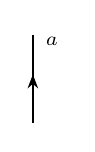
\begin{tikzpicture}\draw[pline] (0,0) -- (0,1.4); \node[dlab,right] at (0.05,1.3) {$a$};\end{tikzpicture} &
    \begin{tikzpicture}\draw[hline] (0,0) -- (0,1.4); \node[dlab,right] at (0.05,1.3) {$i$};\end{tikzpicture} &
    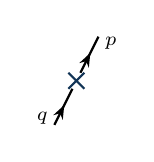
\begin{tikzpicture}\node[fvtx] (f) at (0,0.7) {}; \draw[pline] (-0.35,0) -- (f); \draw[pline] (f) -- (0.35,1.4);
      \node[dlab,right] at (0.3,1.3) {$p$}; \node[dlab,left] at (-0.3,0.1) {$q$};\end{tikzpicture} &
    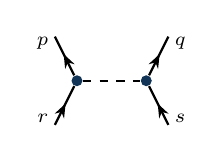
\begin{tikzpicture}\node[vtx] (v1) at (0,0.7) {}; \node[vtx] (v2) at (1.1,0.7) {}; \draw[vint] (v1) -- (v2);
      \draw[pline] (-0.35,0) -- (v1); \draw[pline] (v1) -- (-0.35,1.4); \draw[pline] (1.45,0) -- (v2); \draw[pline] (v2) -- (1.45,1.4);
      \node[dlab,left] at (-0.3,1.3) {$p$}; \node[dlab,left] at (-0.3,0.1) {$r$}; \node[dlab,right] at (1.4,1.3) {$q$}; \node[dlab,right] at (1.4,0.1) {$s$};\end{tikzpicture}\\
    particle line, arrow up & hole line, arrow down & $f_{pq}$: one line in, one out & $\element{pq}{v}{rs}$: two vertices\\[0.4em]
    \multicolumn{2}{c}{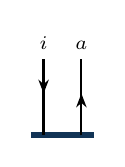
\begin{tikzpicture}
      \draw[amp] (-0.5,0) -- (0.5,0);
      \draw[hline] (-0.3,0) -- (-0.3,1.2); \draw[pline] (0.3,0) -- (0.3,1.2);
      \node[dlab,above] at (-0.3,1.2) {$i$}; \node[dlab,above] at (0.3,1.2) {$a$};
    \end{tikzpicture}} &
    \multicolumn{2}{c}{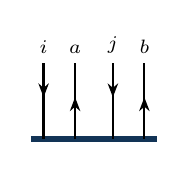
\begin{tikzpicture}
      \draw[amp] (-1.0,0) -- (1.0,0);
      \draw[hline] (-0.8,0) -- (-0.8,1.2); \draw[pline] (-0.3,0) -- (-0.3,1.2);
      \draw[hline] (0.3,0) -- (0.3,1.2); \draw[pline] (0.8,0) -- (0.8,1.2);
      \node[dlab,above] at (-0.8,1.2) {$i$}; \node[dlab,above] at (-0.3,1.2) {$a$}; \node[dlab,above] at (0.3,1.2) {$j$}; \node[dlab,above] at (0.8,1.2) {$b$};
    \end{tikzpicture}}\\
    \multicolumn{2}{c}{$C_i^a$: a bar with one hole and one particle line} & \multicolumn{2}{c}{$C_{ij}^{ab}$: two pairs; $C_3$ three, and so on}
  \end{tabular}
  \end{center}
  \begin{itemize}
    \item An amplitude $C_n$ is a bar from which $n$ particle-hole pairs emerge; $\hat{V}_N$ a dashed line joining two vertices, each with one line in and one out, read as $\element{\text{out}_1\,\text{out}_2}{v}{\text{in}_1\,\text{in}_2}$ (antisymmetrised); $\hat{F}_N$ a cross, $f_{\text{out},\text{in}}$.
    \item The bra $\bra{\Phi_H^P}$ fixes the \alert{open lines at the top}: none for the energy equation, one pair $(a,i)$ for the singles, two pairs for the doubles; every other line is internal and summed over. A term of the equations is one way of joining the open lines, one piece of $\hat{H}$ and one bar with \emph{every} line of $\hat{H}$ and of the bar connected -- the generalised Wick theorem, drawn.
  \end{itemize}
\end{frame}

\begin{frame}{The energy equation, drawn}
  \footnotesize
  \[
    \Delta E=
    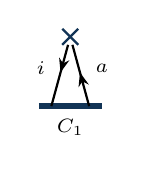
\begin{tikzpicture}
      \draw[amp] (-0.5,0) -- (0.5,0); \node[dlab,below] at (0,-0.05) {$C_1$};
      \node[fvtx] (f) at (0,1.1) {};
      \draw[hline] (-0.3,0) -- (f); \draw[pline] (0.3,0) -- (f);
      \node[dlab,left] at (-0.25,0.6) {$i$}; \node[dlab,right] at (0.25,0.6) {$a$};
    \end{tikzpicture}
    \;+\;
    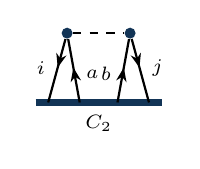
\begin{tikzpicture}
      \draw[amp] (-1.0,0) -- (1.0,0); \node[dlab,below] at (0,-0.05) {$C_2$};
      \node[vtx] (v1) at (-0.5,1.1) {}; \node[vtx] (v2) at (0.5,1.1) {}; \draw[vint] (v1) -- (v2);
      \draw[hline] (-0.8,0) -- (v1); \draw[pline] (-0.3,0) -- (v1);
      \draw[pline] (0.3,0) -- (v2); \draw[hline] (0.8,0) -- (v2);
      \node[dlab,left] at (-0.7,0.55) {$i$}; \node[dlab,right] at (-0.35,0.45) {$a$};
      \node[dlab,left] at (0.35,0.45) {$b$}; \node[dlab,right] at (0.7,0.55) {$j$};
    \end{tikzpicture}
    \;=\;\sum_{ia}f_{ia}C_i^a+\frac14\sum_{ijab}\element{ij}{\hat{v}}{ab}C_{ij}^{ab}.
  \]
  \begin{block}{Rules for the value of a diagram}
    \begin{enumerate}
      \item Sum over all internal labels; write $f_{\text{out},\text{in}}$ for every cross, $\element{\text{out}\,\text{out}}{v}{\text{in}\,\text{in}}$ for every interaction, and the amplitude of every bar.
      \item A factor $\frac12$ for each pair of \alert{equivalent lines}: two lines of the same kind joining the same two elements in the same direction.
      \item A sign $(-1)^{h+l}$, $h$ the number of hole lines, $l$ the number of closed loops -- for open diagrams counting the \emph{quasi-loops} obtained by joining each open particle line to its partner hole line at the top.
      \item For open diagrams, a permutation operator $P$ for each pair of open lines that are \emph{not} equivalent.
    \end{enumerate}
  \end{block}
  \vspace{-0.3em}First diagram: $h=1$, $l=1$, no equivalent lines: $+f_{ia}C_i^a$. Second: $h=2$, $l=2$, two equivalent pairs ($i,j$ and $a,b$): $+\frac14\element{ij}{v}{ab}C_{ij}^{ab}$. \checkmark
\end{frame}

\begin{frame}{The singles equation, drawn: the $\hat{C}_1$ terms}
  \small
  \tikzset{every picture/.style={scale=1.0,baseline=(current bounding box.center)}}
  Open lines $a$ (up) and $i$ (down) at the top; $\Delta E\,C_i^a=$
  \[
    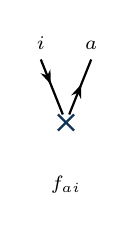
\begin{tikzpicture}
      \node[fvtx] (f) at (0,0.4) {};
      \draw[hline] (f) -- (-0.4,1.4); \draw[pline] (f) -- (0.4,1.4);
      \node[dlab,above] at (-0.4,1.4) {$i$}; \node[dlab,above] at (0.4,1.4) {$a$};
      \node[dlab,below] at (0,-0.3) {$f_{ai}$};
    \end{tikzpicture}
    \;+\;
    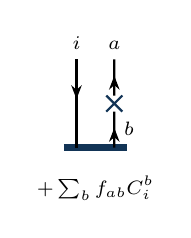
\begin{tikzpicture}
      \draw[amp] (-0.5,0) -- (0.5,0);
      \draw[hline] (-0.3,0) -- (-0.3,1.4);
      \node[fvtx] (f) at (0.3,0.7) {}; \draw[pline] (0.3,0) -- (f); \draw[pline] (f) -- (0.3,1.4);
      \node[dlab,above] at (-0.3,1.4) {$i$}; \node[dlab,above] at (0.3,1.4) {$a$}; \node[dlab,right] at (0.3,0.3) {$b$};
      \node[dlab,below] at (0,-0.3) {$+\sum_bf_{ab}C_i^b$};
    \end{tikzpicture}
    \;+\;
    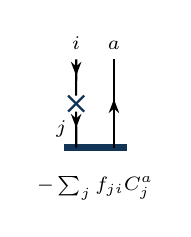
\begin{tikzpicture}
      \draw[amp] (-0.5,0) -- (0.5,0);
      \node[fvtx] (f) at (-0.3,0.7) {}; \draw[hline] (-0.3,0) -- (f); \draw[hline] (f) -- (-0.3,1.4);
      \draw[pline] (0.3,0) -- (0.3,1.4);
      \node[dlab,above] at (-0.3,1.4) {$i$}; \node[dlab,above] at (0.3,1.4) {$a$}; \node[dlab,left] at (-0.3,0.3) {$j$};
      \node[dlab,below] at (0,-0.3) {$-\sum_jf_{ji}C_j^a$};
    \end{tikzpicture}
    \;+\;
    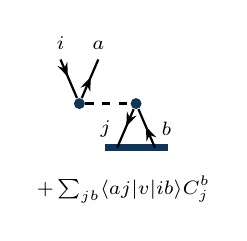
\begin{tikzpicture}
      \draw[amp] (-0.1,0) -- (0.9,0);
      \node[vtx] (v1) at (-0.5,0.7) {}; \node[vtx] (v2) at (0.4,0.7) {}; \draw[vint] (v1) -- (v2);
      \draw[hline] (v1) -- (-0.8,1.4); \draw[pline] (v1) -- (-0.2,1.4);
      \draw[hline] (0.1,0) -- (v2); \draw[pline] (0.7,0) -- (v2);
      \node[dlab,above] at (-0.8,1.4) {$i$}; \node[dlab,above] at (-0.2,1.4) {$a$};
      \node[dlab,left] at (0.15,0.3) {$j$}; \node[dlab,right] at (0.65,0.3) {$b$};
      \node[dlab,below] at (0.2,-0.3) {$+\sum_{jb}\element{aj}{v}{ib}C_j^b$};
    \end{tikzpicture}
    \;+\;\cdots
  \]
  \vspace{0.4em}
  \begin{itemize}
    \item Diagram 1: the driving term, $h=1$, $l=1$ (the quasi-loop $a$--$i$): $+f_{ai}$. Diagram 2: the cross on the particle line, $h=1$, $l=1$: $+f_{ab}C_i^b$. Diagram 3: the cross on the hole line, $h=2$ ($i$ and $j$), $l=1$: $-f_{ji}C_j^a$. Diagram 4: the bar closes a \emph{bubble} $(j,b)$ on one vertex, the other vertex carries the open lines: $h=2$, $l=2$: $+\element{aj}{v}{ib}C_j^b$.
    \item In a Hartree-Fock basis diagram 1 is absent and diagrams 2, 3 collapse to $(\varepsilon_a-\varepsilon_i)C_i^a$: the ``energy denominator'' of perturbation theory is the crosses on the open lines.
  \end{itemize}
\end{frame}

\begin{frame}{The singles equation, drawn: the $\hat{C}_2$ and $\hat{C}_3$ terms}
  \small
  \[
    \cdots\;+\;
    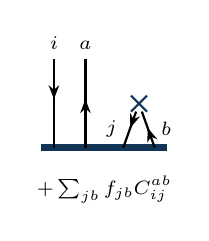
\begin{tikzpicture}
      \draw[amp] (-1.0,0) -- (1.0,0);
      \draw[hline] (-0.8,0) -- (-0.8,1.4); \draw[pline] (-0.3,0) -- (-0.3,1.4);
      \node[fvtx] (f) at (0.55,0.7) {}; \draw[hline] (0.3,0) -- (f); \draw[pline] (0.8,0) -- (f);
      \node[dlab,above] at (-0.8,1.4) {$i$}; \node[dlab,above] at (-0.3,1.4) {$a$};
      \node[dlab,left] at (0.35,0.3) {$j$}; \node[dlab,right] at (0.75,0.3) {$b$};
      \node[dlab,below] at (0,-0.3) {$+\sum_{jb}f_{jb}C_{ij}^{ab}$};
    \end{tikzpicture}
    \;+\;
    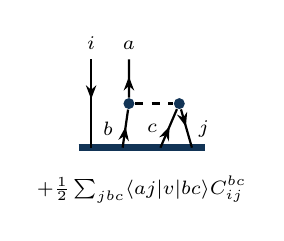
\begin{tikzpicture}
      \draw[amp] (-1.0,0) -- (1.0,0);
      \draw[hline] (-0.8,0) -- (-0.8,1.4);
      \node[vtx] (v1) at (-0.2,0.7) {}; \node[vtx] (v2) at (0.6,0.7) {}; \draw[vint] (v1) -- (v2);
      \draw[pline] (-0.3,0) -- (v1); \draw[pline] (v1) -- (-0.2,1.4);
      \draw[pline] (0.3,0) -- (v2); \draw[hline] (0.8,0) -- (v2);
      \node[dlab,above] at (-0.8,1.4) {$i$}; \node[dlab,above] at (-0.2,1.4) {$a$};
      \node[dlab,left] at (-0.3,0.3) {$b$}; \node[dlab,left] at (0.4,0.3) {$c$}; \node[dlab,right] at (0.75,0.3) {$j$};
      \node[dlab,below] at (0,-0.3) {$+\frac12\sum_{jbc}\element{aj}{v}{bc}C_{ij}^{bc}$};
    \end{tikzpicture}
    \;+\;
    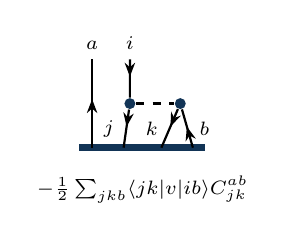
\begin{tikzpicture}
      \draw[amp] (-1.0,0) -- (1.0,0);
      \draw[pline] (-0.8,0) -- (-0.8,1.4);
      \node[vtx] (v1) at (-0.2,0.7) {}; \node[vtx] (v2) at (0.6,0.7) {}; \draw[vint] (v1) -- (v2);
      \draw[hline] (-0.3,0) -- (v1); \draw[hline] (v1) -- (-0.2,1.4);
      \draw[hline] (0.3,0) -- (v2); \draw[pline] (0.8,0) -- (v2);
      \node[dlab,above] at (-0.8,1.4) {$a$}; \node[dlab,above] at (-0.2,1.4) {$i$};
      \node[dlab,left] at (-0.3,0.3) {$j$}; \node[dlab,left] at (0.4,0.3) {$k$}; \node[dlab,right] at (0.75,0.3) {$b$};
      \node[dlab,below] at (0,-0.3) {$-\frac12\sum_{jkb}\element{jk}{v}{ib}C_{jk}^{ab}$};
    \end{tikzpicture}
    \;+\;
    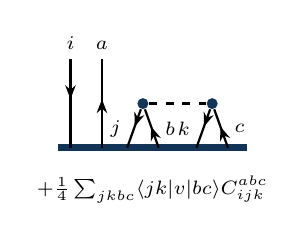
\begin{tikzpicture}
      \draw[amp] (-1.5,0) -- (1.5,0);
      \draw[hline] (-1.3,0) -- (-1.3,1.4); \draw[pline] (-0.8,0) -- (-0.8,1.4);
      \node[vtx] (v1) at (-0.15,0.7) {}; \node[vtx] (v2) at (0.95,0.7) {}; \draw[vint] (v1) -- (v2);
      \draw[hline] (-0.4,0) -- (v1); \draw[pline] (0.1,0) -- (v1);
      \draw[hline] (0.7,0) -- (v2); \draw[pline] (1.2,0) -- (v2);
      \node[dlab,above] at (-1.3,1.4) {$i$}; \node[dlab,above] at (-0.8,1.4) {$a$};
      \node[dlab,left] at (-0.35,0.3) {$j$}; \node[dlab,right] at (0.05,0.3) {$b$}; \node[dlab,left] at (0.75,0.3) {$k$}; \node[dlab,right] at (1.15,0.3) {$c$};
      \node[dlab,below] at (0,-0.3) {$+\frac14\sum_{jkbc}\element{jk}{v}{bc}C_{ijk}^{abc}$};
    \end{tikzpicture}
  \]
  \vspace{0.4em}
  \begin{itemize}
    \item Diagram 5: a bubble on the cross, $h=2$, $l=2$: $+$. Diagram 6: two particle lines $b,c$ from the bar into the interaction, equivalent ($\frac12$); $h=2$, $l=2$: $+$. Diagram 7: its mirror image with two equivalent hole lines; $h=3$, $l=2$: $-$. Diagram 8: two bubbles on the two vertices, two equivalent pairs ($\frac14$); $h=3$, $l=3$: $+$.
    \item Every diagram is \alert{connected} to the open lines: in the singles equation there is no room for a disconnected piece. That changes for the doubles.
  \end{itemize}
\end{frame}

\begin{frame}{The doubles equation, drawn}
  \footnotesize
  \tikzset{every picture/.style={scale=0.66,baseline=(current bounding box.center)}}
  \vspace{-0.4em}Open lines $a,b$ (up) and $i,j$ (down); the driving term, the five doubles-doubles diagrams, and the disconnected singles term:
  \begin{center}
    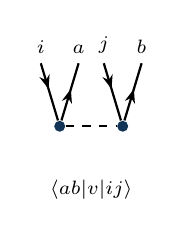
\begin{tikzpicture}
      \node[vtx] (v1) at (-0.5,0.4) {}; \node[vtx] (v2) at (0.5,0.4) {}; \draw[vint] (v1) -- (v2);
      \draw[hline] (v1) -- (-0.8,1.4); \draw[pline] (v1) -- (-0.2,1.4); \draw[hline] (v2) -- (0.2,1.4); \draw[pline] (v2) -- (0.8,1.4);
      \node[dlab,above] at (-0.8,1.4) {$i$}; \node[dlab,above] at (-0.2,1.4) {$a$}; \node[dlab,above] at (0.2,1.4) {$j$}; \node[dlab,above] at (0.8,1.4) {$b$};
      \node[dlab,below] at (0,-0.3) {$\element{ab}{v}{ij}$};
    \end{tikzpicture}
    \;
    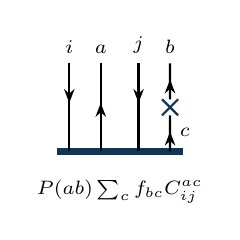
\begin{tikzpicture}
      \draw[amp] (-1.0,0) -- (1.0,0);
      \draw[hline] (-0.8,0) -- (-0.8,1.4); \draw[pline] (-0.3,0) -- (-0.3,1.4); \draw[hline] (0.3,0) -- (0.3,1.4);
      \node[fvtx] (f) at (0.8,0.7) {}; \draw[pline] (0.8,0) -- (f); \draw[pline] (f) -- (0.8,1.4);
      \node[dlab,above] at (-0.8,1.4) {$i$}; \node[dlab,above] at (-0.3,1.4) {$a$}; \node[dlab,above] at (0.3,1.4) {$j$}; \node[dlab,above] at (0.8,1.4) {$b$}; \node[dlab,right] at (0.8,0.3) {$c$};
      \node[dlab,below] at (0,-0.3) {$P(ab)\sum_cf_{bc}C_{ij}^{ac}$};
    \end{tikzpicture}
    \;
    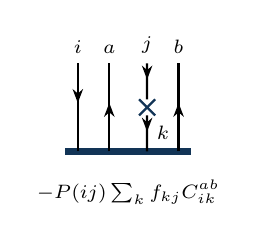
\begin{tikzpicture}
      \draw[amp] (-1.0,0) -- (1.0,0);
      \draw[hline] (-0.8,0) -- (-0.8,1.4); \draw[pline] (-0.3,0) -- (-0.3,1.4); \draw[pline] (0.8,0) -- (0.8,1.4);
      \node[fvtx] (f) at (0.3,0.7) {}; \draw[hline] (0.3,0) -- (f); \draw[hline] (f) -- (0.3,1.4);
      \node[dlab,above] at (-0.8,1.4) {$i$}; \node[dlab,above] at (-0.3,1.4) {$a$}; \node[dlab,above] at (0.3,1.4) {$j$}; \node[dlab,above] at (0.8,1.4) {$b$}; \node[dlab,right] at (0.3,0.3) {$k$};
      \node[dlab,below] at (0,-0.3) {$-P(ij)\sum_kf_{kj}C_{ik}^{ab}$};
    \end{tikzpicture}
    \;
    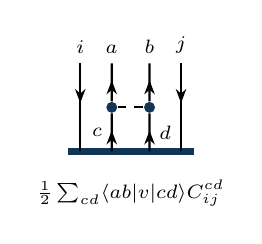
\begin{tikzpicture}
      \draw[amp] (-1.0,0) -- (1.0,0);
      \draw[hline] (-0.8,0) -- (-0.8,1.4); \draw[hline] (0.8,0) -- (0.8,1.4);
      \node[vtx] (v1) at (-0.3,0.7) {}; \node[vtx] (v2) at (0.3,0.7) {}; \draw[vint] (v1) -- (v2);
      \draw[pline] (-0.3,0) -- (v1); \draw[pline] (v1) -- (-0.3,1.4); \draw[pline] (0.3,0) -- (v2); \draw[pline] (v2) -- (0.3,1.4);
      \node[dlab,above] at (-0.8,1.4) {$i$}; \node[dlab,above] at (-0.3,1.4) {$a$}; \node[dlab,above] at (0.3,1.4) {$b$}; \node[dlab,above] at (0.8,1.4) {$j$};
      \node[dlab,left] at (-0.3,0.3) {$c$}; \node[dlab,right] at (0.3,0.3) {$d$};
      \node[dlab,below] at (0,-0.3) {$\frac12\sum_{cd}\element{ab}{v}{cd}C_{ij}^{cd}$};
    \end{tikzpicture}\\[0.1em]
    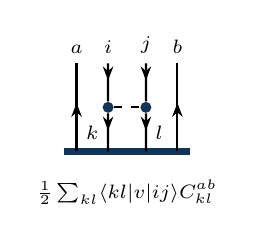
\begin{tikzpicture}
      \draw[amp] (-1.0,0) -- (1.0,0);
      \draw[pline] (-0.8,0) -- (-0.8,1.4); \draw[pline] (0.8,0) -- (0.8,1.4);
      \node[vtx] (v1) at (-0.3,0.7) {}; \node[vtx] (v2) at (0.3,0.7) {}; \draw[vint] (v1) -- (v2);
      \draw[hline] (-0.3,0) -- (v1); \draw[hline] (v1) -- (-0.3,1.4); \draw[hline] (0.3,0) -- (v2); \draw[hline] (v2) -- (0.3,1.4);
      \node[dlab,above] at (-0.8,1.4) {$a$}; \node[dlab,above] at (-0.3,1.4) {$i$}; \node[dlab,above] at (0.3,1.4) {$j$}; \node[dlab,above] at (0.8,1.4) {$b$};
      \node[dlab,left] at (-0.3,0.3) {$k$}; \node[dlab,right] at (0.3,0.3) {$l$};
      \node[dlab,below] at (0,-0.3) {$\frac12\sum_{kl}\element{kl}{v}{ij}C_{kl}^{ab}$};
    \end{tikzpicture}
    \;
    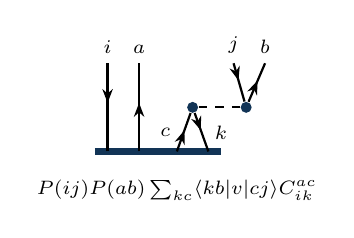
\begin{tikzpicture}
      \draw[amp] (-1.0,0) -- (1.0,0);
      \draw[hline] (-0.8,0) -- (-0.8,1.4); \draw[pline] (-0.3,0) -- (-0.3,1.4);
      \node[vtx] (v1) at (0.55,0.7) {}; \node[vtx] (v2) at (1.4,0.7) {}; \draw[vint] (v1) -- (v2);
      \draw[pline] (0.3,0) -- (v1); \draw[hline] (0.8,0) -- (v1);
      \draw[hline] (v2) -- (1.2,1.4); \draw[pline] (v2) -- (1.7,1.4);
      \node[dlab,above] at (-0.8,1.4) {$i$}; \node[dlab,above] at (-0.3,1.4) {$a$}; \node[dlab,above] at (1.2,1.4) {$j$}; \node[dlab,above] at (1.7,1.4) {$b$};
      \node[dlab,left] at (0.35,0.3) {$c$}; \node[dlab,right] at (0.75,0.3) {$k$};
      \node[dlab,below] at (0.3,-0.3) {$P(ij)P(ab)\sum_{kc}\element{kb}{v}{cj}C_{ik}^{ac}$};
    \end{tikzpicture}
    \qquad
    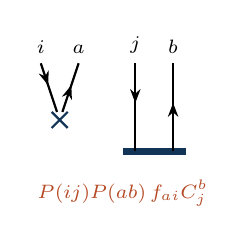
\begin{tikzpicture}
      \node[fvtx] (f) at (-1.0,0.5) {};
      \draw[hline] (f) -- (-1.3,1.4); \draw[pline] (f) -- (-0.7,1.4);
      \node[dlab,above] at (-1.3,1.4) {$i$}; \node[dlab,above] at (-0.7,1.4) {$a$};
      \draw[amp] (0.0,0) -- (1.0,0);
      \draw[hline] (0.2,0) -- (0.2,1.4); \draw[pline] (0.8,0) -- (0.8,1.4);
      \node[dlab,above] at (0.2,1.4) {$j$}; \node[dlab,above] at (0.8,1.4) {$b$};
      \node[dlab,below] at (0,-0.3) {\color{warm}$P(ij)P(ab)\,f_{ai}C_j^b$};
    \end{tikzpicture}
  \end{center}
  \vspace{-0.3em}
  \begin{itemize}
    \item Crosses on an open line, particle and hole ladders ($\frac12$ per equivalent pair), a ring with four inequivalent open lines ($P(ij)P(ab)$): with the driving term, this is CID -- and the linear part of coupled cluster.
    \item The last diagram is \alert{two pieces}, the open $f_{ai}$ vertex beside a $C_1$ bar: disconnected. The linked-cluster theorem removes such terms; CI keeps them and pays with size consistency.
  \end{itemize}
\end{frame}

\begin{frame}{Pause to think: from diagram to term and back}
  \thinkq{4}{
  \begin{enumerate}
    \item Write down the value of the diagram below (open lines $a$, $i$) using the four rules, and identify it in the singles equation.
    \[
      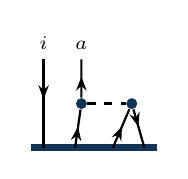
\begin{tikzpicture}
        \draw[amp] (-1.0,0) -- (1.0,0);
        \draw[hline] (-0.8,0) -- (-0.8,1.4);
        \node[vtx] (v1) at (-0.2,0.7) {}; \node[vtx] (v2) at (0.6,0.7) {}; \draw[vint] (v1) -- (v2);
        \draw[pline] (-0.3,0) -- (v1); \draw[pline] (v1) -- (-0.2,1.4);
        \draw[pline] (0.3,0) -- (v2); \draw[hline] (0.8,0) -- (v2);
        \node[dlab,above] at (-0.8,1.4) {$i$}; \node[dlab,above] at (-0.2,1.4) {$a$};
      \end{tikzpicture}
    \]
    \item Draw the diagram for $-\frac12P(ij)\sum_{klc}\element{kl}{\hat{v}}{jc}C_{ikl}^{abc}$ in the doubles equation and check its sign and factor with the rules.
    \item Which diagrams of the singles equation survive if the amplitudes are those of CID ($C_1=C_3=0$)? What does the singles equation then say?
  \end{enumerate}}
\end{frame}

\begin{frame}{Answer}
  \thinka{
  \begin{enumerate}
    \item A $C_2$ bar with $i$ open, particles $b,c$ into the two vertices, hole $j$ from the right vertex back to the bar, $a$ emitted by the left vertex: $\element{aj}{v}{bc}C_{ij}^{bc}$ summed over $j,b,c$; $b,c$ equivalent: $\frac12$; $h=2$, loops $b\to a\to i\to$bar and $c\to j\to$bar: $l=2$, sign $+$. Diagram 6.
    \item A $C_3$ bar with open $a$, $b$, $i$; holes $k,l$ from the bar into the two vertices; one vertex re-emits the open hole $j$, the other absorbs the particle $c$. Equivalent $k,l$: $\frac12$; open holes $i,j$ inequivalent: $P(ij)$; $h=4$, loops $a$--$i$, $b$--$j$ (through $l$), $k$--$c$: $l=3$, sign $(-1)^7=-1$. \checkmark
    \item Diagrams 1, 5, 6, 7 -- four terms and no $C_i^a$ on the left; $f_{ai}+\sum f_{jb}C_{ij}^{ab}+\dots\neq0$ in general. CID does not solve the singles rows, it \emph{drops} them: Ritz in a subspace projects onto the subspace and satisfies only its own rows.
  \end{enumerate}}
\end{frame}

\begin{frame}{A non-practical way of solving the FCI equations (\texttt{fci.do.txt}, section 5.10)}
  \footnotesize
  Take the singles equation and isolate the diagonal term: $\bra{\Phi_i^a}\hat{H}\ket{\Phi_i^a}=E_{\mathrm{ref}}+f_{aa}-f_{ii}-\element{ai}{v}{ai}\equiv H_{ia,ia}$, so that
  \[
    \bigl(E-H_{ia,ia}\bigr)C_i^a=f_{ai}+\sum_{bj\neq ai}\bra{\Phi_i^a}\hat{H}\ket{\Phi_j^b}C_j^b+\sum_{bcjk}\bra{\Phi_i^a}\hat{H}\ket{\Phi_{jk}^{bc}}C_{jk}^{bc}+\sum_{bcdjkl}\bra{\Phi_i^a}\hat{H}\ket{\Phi_{jkl}^{bcd}}C_{jkl}^{bcd},
  \]
  and likewise for every other row. A prescription:
  \begin{block}{Iteration}
    \begin{enumerate}
      \item Guess the amplitudes -- from first-order perturbation theory, $C_i^a=f_{ai}/(\varepsilon_i-\varepsilon_a)$, $C_{ij}^{ab}=\element{ab}{v}{ij}/(\varepsilon_i+\varepsilon_j-\varepsilon_a-\varepsilon_b)$.
      \item Compute $E$ from the energy equation, $E=E_{\mathrm{ref}}+\sum f_{ia}C_i^a+\frac14\sum\element{ij}{v}{ab}C_{ij}^{ab}$.
      \item Compute the right-hand side of every row with the current amplitudes, divide by $E-H_{K,K}$, update every $C_K$; repeat from 2 until nothing moves.
    \end{enumerate}
  \end{block}
  \begin{itemize}
    \item The right-hand sides are the diagrams of the previous slides; $E$ on the left makes the scheme \alert{non-linear} in the amplitudes although each row is linear. Pairing model, four levels (section 7 of the notebook): the \alert{first iterate is exactly} $E_{\mathrm{ref}}-\frac{7}{24}g^2$, the second-order energy of pause \#2; at $g=1$ the sequence $0.7083$, $0.6359$ ($5$ iterations), $0.63554847$ ($20$) reaches the FCI value.
  \end{itemize}
\end{frame}

\begin{frame}{What the iteration is, and what it is not}
  \footnotesize
  \begin{itemize}
    \item A Jacobi iteration on $\bm{H}\bm{C}=E\bm{C}$ with the energy updated on the way. It converges when the reference dominates the ground state, and it produces, order by order, the \alert{perturbation series}: the $m$-th iterate contains the right-hand side substituted into itself $m$ times -- chapter 7 does the bookkeeping, with the same diagrams and energy denominators from the crosses on the open lines.
    \item \emph{Not} a way around the wall: the loop runs over all $\binom{n}{N}$ amplitudes and every right-hand side costs as much as $\hat{H}\ket{\Phi}$. Lanczos does the same work far more cleverly.
    \item It \emph{is} the template for every practical method -- each a rule for which rows and diagrams to keep, and how to close the system:
  \end{itemize}
  \vspace{-0.4em}
  \begin{center}\scriptsize
  \renewcommand{\arraystretch}{1.1}
  \begin{tabular}{lll}
    \toprule
    method & amplitudes & how the equations are closed\\
    \midrule
    Hartree-Fock & none: $C_0$ only & vary the \emph{orbitals} until $f_{ai}=0$\\
    perturbation theory & all, order by order & a fixed number of iterations, $E\to E_{\mathrm{ref}}$ in the denominators\\
    Tamm-Dancoff, RPA & singles (and ring doubles) & diagonalise the $1p1h$ block; sum the rings\\
    truncated CI & up to a fixed level & Ritz in the subspace: linear, unlinked terms kept\\
    coupled cluster & up to a fixed level & $e^{\hat{T}}$: same diagrams plus non-linear ones; unlinked terms cancel\\
    \bottomrule
  \end{tabular}
  \end{center}
  \vspace{-0.2em}Full CI is the fixed point that measures each answer: whenever a model is small enough to solve exactly, solve it and calibrate.
\end{frame}

\begin{frame}{The link to Hartree-Fock: kill the driving term}
  \footnotesize
  Look at the singles equation once more. Its driving term is $f_{ai}$, the same quantity that couples the reference to the singles in the energy equation:
  \[
    \Delta E=\sum_{ia}f_{ia}C_i^a+\frac14\sum\element{ij}{v}{ab}C_{ij}^{ab},
    \qquad
    \Delta E\,C_i^a=f_{ai}+\sum_bf_{ab}C_i^b-\sum_jf_{ji}C_j^a+\cdots
  \]
  \begin{itemize}
    \item If the single-particle basis could be chosen such that $f_{ai}=0$ for all $a,i$, the singles would be driven by the doubles only, the energy equation would contain the doubles alone, and the reference would be the best single determinant \emph{in the sense of the variational principle}.
    \item That choice exists: the Fock matrix $f_{pq}=h_{pq}+\sum_i\element{pi}{v}{qi}$ depends on the occupied orbitals, and diagonalising it self-consistently -- the occupied orbitals being its own lowest eigenvectors -- makes $f_{ai}=0$. This is the \alert{Hartree-Fock} basis, and $f_{ai}=0$ is \alert{Brillouin's theorem}.
    \item Section 8 of the notebook, random Hamiltonian of yesterday: $E_{\mathrm{ref}}=6.497$, $E^{\mathrm{HF}}=1.298$ after $48$ iterations, $E_0^{\mathrm{FCI}}=0.748$ in \emph{both} bases; in the HF basis $\max|f_{ai}|=9\times10^{-11}$, the $0p0h$--$1p1h$ block is empty and $\Delta E=-0.550$ comes from the doubles term alone.
  \end{itemize}
  \mbbox{\footnotesize Chapter 5 optimised the \emph{expansion} on a fixed reference. Chapter 6 keeps one determinant and optimises the \emph{reference}. Both are the variational principle; the second is the last lecture of this week.}
\end{frame}

\begin{frame}{Summary of lecture 3}
  \begin{itemize}
    \item Projecting $(\hat{H}-E)\ket{\Psi_0}=0$ row by row gives the energy equation ($\Delta E$ from singles and doubles only), the singles equation (eight terms, $C_0$ to $C_3$) and the doubles equation (thirteen terms, $C_0$ to $C_4$) -- every term a product of one $f$ or $v$ and one amplitude, all verified numerically in the notebook.
    \item The same equations are diagrams: bars for amplitudes, crosses and dashed lines for $\hat{F}_N$ and $\hat{V}_N$, open lines from the bra; value by four rules -- sums, $\frac12$ per equivalent pair, $(-1)^{h+l}$, permutations. The doubles equation contains a \alert{disconnected} diagram, the fingerprint of the size-consistency failure.
    \item Iterating the rows from a perturbative guess reproduces second-order perturbation theory at the first step and converges to FCI; every practical method is a rule for which rows and which diagrams to keep.
    \item Making the driving term $f_{ai}$ vanish by choosing the orbitals is Hartree-Fock theory -- next.
  \end{itemize}
\end{frame}

% ======================================================================
\section{Friday, lecture 4: Hartree-Fock theory}
% ======================================================================

\begin{frame}{Why a mean field? (section 6.1)}
  \footnotesize
  Chapter 5 showed that the exact answer is a superposition of exponentially many determinants and that we cannot afford it. Chapter 6 takes the opposite tack: \alert{keep exactly one determinant, and ask which one is best}.
  \begin{block}{Hartree-Fock theory in two ingredients}
    A single-particle basis defined by its own eigenvalue problem,
    \[
      \hat{h}^{\mathrm{HF}}\psi_\alpha=\varepsilon_\alpha\psi_\alpha,\qquad
      \hat{h}^{\mathrm{HF}}=\hat{t}+\hat{u}_{\mathrm{ext}}+\hat{u}^{\mathrm{HF}},
    \]
    and the prescription for the still unknown one-body potential $\hat{u}^{\mathrm{HF}}$: choose it such that $E^{\mathrm{HF}}=\bra{\Phi_0}\hat{H}\ket{\Phi_0}$ is stationary, with $\ket{\Phi_0}$ the determinant of the $N$ lowest solutions.
  \end{block}
  \begin{itemize}
    \item The variational principle guarantees $E^{\mathrm{HF}}\ge E_0$: an upper bound, like every Ritz value of this week -- here with the \emph{orbitals} as parameters and the expansion frozen at one term.
    \item We shall find that $\hat{h}^{\mathrm{HF}}$ is exactly the operator $\hat{f}$ of the normal-ordered Hamiltonian,
    \[
      \element{p}{\hat{h}^{\mathrm{HF}}}{q}=\element{p}{\hat{t}+\hat{u}_{\mathrm{ext}}}{q}+\sum_{i\le F}\element{pi}{\hat{v}}{qi},
      \qquad
      \element{p}{\hat{u}^{\mathrm{HF}}}{q}=\sum_{i\le F}\element{pi}{\hat{v}}{qi}:
    \]
    the interaction summed over the other fermions is an effective one-body field in which a given fermion moves -- dependent on which states are occupied (\alert{medium dependence}) and on the interaction. For atoms and molecules $\hat{u}_{\mathrm{ext}}$ is the attraction of the nuclei; a nucleus has none, and the whole field must be generated self-consistently.
  \end{itemize}
\end{frame}

\begin{frame}{Variational calculus and Lagrange multipliers (section 6.2)}
  \small
  The same machinery as Thursday, in its simplest setting: one particle, $E=\int\psi^{*}\hat{H}\psi\,\dd^3r$ with $\int\psi^{*}\psi\,\dd^3r=1$ and $\hat{H}=-\frac12\nabla^2+V$. Integrating the kinetic term by parts, the constrained variation is
  \[
    \delta\Bigl\{\int\Bigl(\tfrac12\nabla\psi^{*}\cdot\nabla\psi+V\psi^{*}\psi-\lambda\psi^{*}\psi\Bigr)\dd^3r\Bigr\}=0 .
  \]
  With $f=\frac12(\psi_x^{*}\psi_x+\psi_y^{*}\psi_y+\psi_z^{*}\psi_z)+V\psi^{*}\psi-\lambda\psi^{*}\psi$, the Euler-Lagrange equation for $\psi^{*}$,
  \[
    \frac{\partial f}{\partial\psi^{*}}-\frac{\partial}{\partial x}\frac{\partial f}{\partial\psi_x^{*}}-\frac{\partial}{\partial y}\frac{\partial f}{\partial\psi_y^{*}}-\frac{\partial}{\partial z}\frac{\partial f}{\partial\psi_z^{*}}=0
    \qquad\Longrightarrow\qquad
    -\tfrac12\nabla^2\psi+V\psi=\lambda\psi .
  \]
  \begin{itemize}
    \item The multiplier is the energy and the stationarity condition is the Schr\"odinger equation. \alert{The pattern of Thursday}: a constrained variation produces an eigenvalue problem, and the multiplier enforcing normalisation is the eigenvalue. In FCI the unknowns were the coefficients $C_H^P$ and the constraint $\sum|C|^2=1$; here the unknown is a function and the constraint an integral.
    \item In Hartree-Fock the unknowns are $N$ orbitals, the constraints are the $N(N+1)/2$ orthonormality integrals $\braket{i}{j}=\delta_{ij}$, and there will be one multiplier per constraint -- reduced to one per orbital by the freedom of the next slide.
  \end{itemize}
\end{frame}

\begin{frame}{Determinants under a linear change of basis (section 6.3)}
  \small
  A determinant is linear in each column separately,
  \[
    \begin{vmatrix}\alpha_1b_{11}+\alpha_2b_{12} & a_{12}\\ \alpha_1b_{21}+\alpha_2b_{22} & a_{22}\end{vmatrix}
    =\alpha_1\begin{vmatrix}b_{11} & a_{12}\\ b_{21} & a_{22}\end{vmatrix}+\alpha_2\begin{vmatrix}b_{12} & a_{12}\\ b_{22} & a_{22}\end{vmatrix},
    \qquad\text{and in general }\det(\bm{B}\bm{C})=\det\bm{B}\,\det\bm{C}.
  \]
  Expand new orbitals in a fixed orthonormal basis, $\psi_p(x)=\sum_\lambda C_{p\lambda}\phi_\lambda(x)$. The Slater determinant of the $\psi$'s is
  \[
    \frac{1}{\sqrt{N!}}
    \begin{vmatrix}
      \sum_\lambda C_{p\lambda}\phi_\lambda(x_1) & \cdots & \sum_\lambda C_{p\lambda}\phi_\lambda(x_N)\\
      \vdots & & \vdots\\
      \sum_\lambda C_{t\lambda}\phi_\lambda(x_1) & \cdots & \sum_\lambda C_{t\lambda}\phi_\lambda(x_N)
    \end{vmatrix}
    =\det(\bm{C})\,\Phi(\phi),
  \]
  with $\Phi(\phi)$ the determinant of the original basis functions. Two consequences, used constantly:
  \begin{itemize}
    \item \textbf{Orthonormality is preserved by a unitary $\bm{C}$}: $\bm{w}_j^{\dagger}\bm{w}_i=\bm{v}_j^{\dagger}\bm{U}^{\dagger}\bm{U}\bm{v}_i=\delta_{ij}$. A unitary change of coefficients never spoils the basis.
    \item \textbf{A determinant is invariant, up to a phase, under any unitary mixing of its occupied orbitals}: it knows only which $N$-dimensional subspace they span. The Hartree-Fock solution is a statement about a \alert{subspace}; the individual orbitals are fixed only by the convention that the Fock matrix be diagonal -- which is what lets us use one multiplier per orbital.
  \end{itemize}
\end{frame}

\begin{frame}{The energy functional in terms of the coefficients (section 6.4)}
  \footnotesize
  The energy of a single determinant is the functional of week 34, $E_{\mathrm{ref}}$ of week 37:
  \[
    E[\Phi]=\sum_{\mu=1}^{N}\element{\mu}{\hat{h}_0}{\mu}+\frac12\sum_{\mu\nu=1}^{N}\element{\mu\nu}{\hat{v}}{\mu\nu}_{\mathrm{AS}} .
  \]
  Insert $\psi_i=\sum_\alpha C_{i\alpha}\phi_\alpha$ (Greek indices over the whole fixed basis, Latin over the $N$ occupied orbitals):
  \begin{block}{$E$ as a function of the coefficients}
    \[
      E[\Phi^{\mathrm{HF}}]=\sum_{i=1}^{N}\sum_{\alpha\beta}C_{i\alpha}^{*}C_{i\beta}\element{\alpha}{\hat{h}_0}{\beta}
      +\frac12\sum_{i,j=1}^{N}\sum_{\alpha\beta\gamma\delta}C_{i\alpha}^{*}C_{j\beta}^{*}C_{i\gamma}C_{j\delta}\element{\alpha\beta}{\hat{v}}{\gamma\delta}_{\mathrm{AS}} .
    \]
  \end{block}
  \begin{itemize}
    \item The coefficients are not free: $\braket{i}{j}=\delta_{ij}=\sum_\alpha C_{i\alpha}^{*}C_{j\alpha}$. Introduce one multiplier $\epsilon_i$ per occupied orbital and make
    \[
      F[\Phi^{\mathrm{HF}}]=E[\Phi^{\mathrm{HF}}]-\sum_{i=1}^{N}\epsilon_i\sum_\alpha C_{i\alpha}^{*}C_{i\alpha}
    \]
    stationary. As on Thursday, $C$ and $C^{*}$ may be varied independently: $\partial F/\partial C_{i\alpha}^{*}=0$.
    \item Compare with FCI: there $E$ was \emph{quadratic} in the unknowns and the stationarity condition linear (an eigenvalue problem). Here $E$ is \emph{quartic} in the $C$'s, and the condition will be an eigenvalue problem whose matrix depends on its own solution.
  \end{itemize}
\end{frame}

\begin{frame}{Carrying out the variation}
  \footnotesize
  Differentiate with respect to $C_{i\alpha}^{*}$. The one-body term gives $\sum_\beta C_{i\beta}\element{\alpha}{\hat{h}_0}{\beta}$. In the two-body term $C_{i\alpha}^{*}$ appears twice -- as $C_{i\alpha}^{*}$ and as $C_{j\beta}^{*}$ with $j=i$ -- with equal contributions by the symmetry of $\element{\alpha\beta}{\hat{v}}{\gamma\delta}_{\mathrm{AS}}$ under the simultaneous interchange of both pairs; they cancel the $\frac12$:
  \[
    \sum_\beta C_{i\beta}\element{\alpha}{\hat{h}_0}{\beta}
    +\sum_{j=1}^{N}\sum_{\beta\gamma\delta}C_{j\beta}^{*}C_{j\delta}C_{i\gamma}\element{\alpha\beta}{\hat{v}}{\gamma\delta}_{\mathrm{AS}}
    =\epsilon_i^{\mathrm{HF}}C_{i\alpha} .
  \]
  Relabel the dummy indices so that $C_{i\beta}$ factors out of both terms, $\sum_\beta\{\element{\alpha}{\hat{h}_0}{\beta}+\sum_{j\gamma\delta}C_{j\gamma}^{*}C_{j\delta}\element{\alpha\gamma}{\hat{v}}{\beta\delta}_{\mathrm{AS}}\}C_{i\beta}=\epsilon_i^{\mathrm{HF}}C_{i\alpha}$:
  \begin{block}{The Hartree-Fock equations}
    \[
      \boxed{\;\sum_\beta h^{\mathrm{HF}}_{\alpha\beta}C_{i\beta}=\epsilon_i^{\mathrm{HF}}C_{i\alpha}\;}
      \qquad
      h^{\mathrm{HF}}_{\alpha\beta}=\element{\alpha}{\hat{h}_0}{\beta}+\sum_{j=1}^{N}\sum_{\gamma\delta}C_{j\gamma}^{*}C_{j\delta}\element{\alpha\gamma}{\hat{v}}{\beta\delta}_{\mathrm{AS}} .
    \]
  \end{block}
  \begin{itemize}
    \item A Hermitian eigenvalue problem, $\bm{h}^{\mathrm{HF}}\bm{C}=\bm{\epsilon}^{\mathrm{HF}}\bm{C}$, with the one complication that \alert{the matrix depends on its own eigenvectors}. In the eigenbasis of $\hat{h}_0$ the first term is $\varepsilon_\alpha\delta_{\alpha\beta}$. No integrals are recomputed: $\element{\alpha}{\hat{h}_0}{\beta}$ and $\element{\alpha\gamma}{\hat{v}}{\beta\delta}_{\mathrm{AS}}$ are tabulated once ($n^4$ storage), each iteration is a contraction with the current coefficients and a diagonalisation.
  \end{itemize}
\end{frame}

\begin{frame}{The density matrix and the self-consistent field (section 6.5)}
  \footnotesize
  The double sum over occupied orbitals enters only through the one-body \alert{density matrix}
  \[
    \rho_{\gamma\delta}=\sum_{i=1}^{N}\braket{\gamma}{i}\braket{i}{\delta}=\sum_{i=1}^{N}C_{i\gamma}C_{i\delta}^{*},
    \qquad
    \bm{\rho}^2=\bm{\rho},\quad\tr\bm{\rho}=N,
    \qquad
    h^{\mathrm{HF}}_{\alpha\beta}=\varepsilon_\alpha\delta_{\alpha\beta}+\sum_{\gamma\delta}\rho_{\gamma\delta}\element{\alpha\gamma}{\hat{v}}{\beta\delta}_{\mathrm{AS}},
  \]
  the projector onto the occupied subspace (the invariance of section 6.3, formalised).
  \begin{block}{The self-consistent field algorithm}
    \begin{enumerate}
      \item Start from a guess, conventionally $C^{(0)}_{i\alpha}=\delta_{i\alpha}$ (the $N$ lowest eigenstates of $\hat{h}_0$); random orthonormal vectors also work.
      \item Build $\bm{\rho}$ and $\bm{h}^{\mathrm{HF}}$; diagonalise; take the $N$ lowest eigenvectors as the new occupied orbitals.
      \item Repeat until the single-particle energies stop moving, $\frac1m\sum_p|\epsilon_p^{(n)}-\epsilon_p^{(n-1)}|\le\lambda\sim10^{-8}$.
    \end{enumerate}
  \end{block}
  \begin{itemize}
    \item \texttt{hartreefock.py}, spinless fermions in a one-dimensional oscillator trap with a softened Coulomb repulsion, eight orbitals: $N=4$ goes from $11.77084712$ to $E^{\mathrm{HF}}=11.62305385$ in $17$ iterations; the first diagonalisation gives $96\%$ of the gain.
    \item \alert{Never use the energy as the convergence criterion.} At a stationary point the energy is quadratic in the orbital displacement: a drift of $10^{-5}$ in the $\epsilon_p$ is $10^{-10}$ in $E$. Everything that depends on the orbitals -- $f_{ai}$, transition elements, the input of a coupled-cluster calculation -- is only as good as the orbital drift (Figure 6.1: linear convergence, a factor four per iteration).
  \end{itemize}
\end{frame}

\begin{frame}{Brillouin's theorem, and FCI in the Hartree-Fock basis}
  \footnotesize
  At convergence the Fock matrix is diagonal in its own eigenbasis, so its occupied-unoccupied block vanishes:
  \[
    f_{ai}=0\qquad\Longleftrightarrow\qquad\bra{\Phi_0}\hat{H}\ket{\Phi_i^a}=0 .
  \]
  The Hartree-Fock solution is \alert{the single-particle basis that decouples the reference from all single excitations}. Section 8 of the notebook, random Hamiltonian, $n=8$, $N=4$ (same $E_0$ in both bases, as it must be):
  \begin{center}\footnotesize
  \renewcommand{\arraystretch}{1.15}
  \begin{tabular}{lrrrrr}
    \toprule
    basis & $E_{\mathrm{ref}}$ or $E^{\mathrm{HF}}$ & CIS & CID & CISD & FCI\\
    \midrule
    eigenstates of $\hat{h}_0$ & $6.497174$ & $2.438662$ & $5.442075$ & $1.157492$ & $0.747713$\\
    Hartree-Fock ($48$ iterations) & $1.298016$ & $1.298016$ & $0.819738$ & $0.774941$ & $0.747713$\\
    \bottomrule
  \end{tabular}
  \end{center}
  \begin{itemize}
    \item In the HF basis $\max|f_{ai}|=9\times10^{-11}$, CIS returns $E^{\mathrm{HF}}$ exactly (Brillouin), the $0p0h$--$1p1h$ block of the FCI matrix is empty, and $\Delta E=-0.550$ is carried by the doubles term of the energy equation alone.
    \item Every truncation is better in the HF basis; the full CI is the same. \alert{The truncations depend on the reference, the exact answer does not} -- which is why Hartree-Fock comes first and every later method is built on it. And $E^{\mathrm{HF}}=\sum_i\epsilon_i^{\mathrm{HF}}-\frac12\sum_{ij}\element{ij}{\hat{v}}{ij}$: the sum of orbital energies double-counts the interaction ($1.29801640$ both ways in the notebook).
  \end{itemize}
\end{frame}

\begin{frame}{Pause to think: when the mean field does nothing}
  \thinkq{3}{
  \begin{enumerate}
    \item For the pairing model with the reference ``levels $1$ and $2$ filled'', write down the Fock matrix $f_{pq}$ (week 37, Example 5). What does the Hartree-Fock iteration do, and what is $E^{\mathrm{HF}}$?
    \item The Hubbard ring in the momentum basis has $f_{ai}=0$ for every $U$ (section 5.7). Is the plane-wave determinant the Hartree-Fock solution? Is it the \emph{best} single determinant?
  \end{enumerate}}
\end{frame}

\begin{frame}{Answer}
  \thinka{
  \begin{enumerate}
    \item $f$ is diagonal: $f_{ii}=\varepsilon_i-g/2$ for the holes (only the partner $\bar\imath$ contributes), $f_{aa}=\varepsilon_a$, $f_{ai}=0$ because the interaction connects pairs to pairs only. The iteration converges at once: the reference \emph{is} the Hartree-Fock determinant, $E^{\mathrm{HF}}=E_{\mathrm{ref}}=2-g$, and the whole correlation energy ($-0.364$ at $g=1$) lies beyond the mean field. The pairing model is built so that Hartree-Fock does nothing and the pair correlations are the entire story.
    \item Yes, and not necessarily. $f_{ai}=0$ is the stationarity condition, so the plane-wave determinant is a Hartree-Fock solution for every $U$ -- by momentum conservation, not by the variation. But stationary is not minimal: at large $U$ a determinant that \emph{breaks} translational symmetry (a spin-density wave, $\uparrow$ and $\downarrow$ alternating on the sites) lies below the Fermi sea, which is then a saddle point. Whether a Hartree-Fock solution is a minimum is the stability question of section 6.10, next week, with the Lipkin model as the worked example.
    \end{enumerate}}
\end{frame}

\begin{frame}{Exercise session: week 38 (suggested set)}
  \footnotesize
  The set combines exercises from the chapter exercise sections of the lecture notes (where full answers are given) with new ones on this week's material. Chapter 5, exercises 1--3 (counting, vanishing blocks, the $6\times6$ pairing matrix) were assigned in week 37; if they were not done, they come first.
  \begin{block}{Exercise 1: bit patterns}
    \begin{enumerate}
      \item[a)] Five orbitals, bits $\alpha_0\dots\alpha_4$. Evaluate $a_3^{\dagger}a_1\ket{01011}$, $a_0^{\dagger}a_4\ket{01101}$ and $a_4^{\dagger}a_3^{\dagger}a_1a_0\ket{11010}$ by anticommuting the operators into place, and again with the ``occupied states strictly between'' rule.
      \item[b)] Show that the phase of $a_j^{\dagger}a_i$ is the product of the phases of $a_i$ and $a_j^{\dagger}$ taken separately, and that it equals $(-1)^{l}$ with $l$ the number of occupied states strictly between $i$ and $j$. Where does the argument use $i\neq j$?
      \item[c)] Count, for $n$ orbitals and $N$ particles, the number of index quadruples for which $a_p^{\dagger}a_q^{\dagger}a_sa_r\ket{\Phi}$ is non-zero, and compare with $n^4$ for $n=40$, $N=8$. Verify with \texttt{apply\_hamiltonian} on random patterns.
    \end{enumerate}
  \end{block}
\end{frame}

\begin{frame}{Exercise session: week 38 (continued)}
  \footnotesize
  \begin{block}{Exercise 2: the FCI equation from the variational principle}
    \begin{enumerate}
      \item[a)] Starting from the Rayleigh quotient $E[\bm{C}]=\bm{C}^{\dagger}\bm{H}\bm{C}/\bm{C}^{\dagger}\bm{C}$, compute $\partial E/\partial C_K^{*}$ and show that the stationary points are the eigenvectors of $\bm{H}$ and the stationary values its eigenvalues. Repeat with a Lagrange multiplier and identify $\lambda=E$.
      \item[b)] For the two-level, one-pair system write down $\det(\bm{H}-E\bm{1})=0$, solve it, expand $E_-$ to order $g^2$ and compare with second-order perturbation theory.
      \item[c)] Compute the characteristic polynomial of the $6\times6$ seniority-zero matrix at $g=1$ (by hand for the trace and the determinant, with \texttt{numpy.poly} for the rest) and verify that its roots are the eigenvalues. Then do the same for the $70\times70$ matrix and explain what you see.
      \item[d)] (Interlacing.) Diagonalise the $6\times6$ matrix in the subspaces $\{\ket{12}\}$, $\{\ket{12},\ket{13}\}$, $\{\ket{12},\ket{13},\ket{14}\}$, \dots\ and verify that every eigenvalue decreases monotonically as the space grows and stays above the corresponding exact eigenvalue.
    \end{enumerate}
  \end{block}
\end{frame}

\begin{frame}{Exercise session: week 38 (continued)}
  \footnotesize
  \begin{block}{Exercise 3 (chapter 5, exercise 4): truncations and size consistency}
    \begin{enumerate}
      \item[a)] Restrict the pairing basis to excitation levels $\le1$ and $\le2$, reproduce the CIS and CID columns, and explain why CIS returns exactly the reference energy.
      \item[b)] Build two non-interacting two-level pairing systems; show that full CI gives twice the energy of one while CID does not (tabulate the error for $g=0.25,0.5,1$); identify the missing configuration, show that quadruples restore the exact result and that $\exp(\hat{T}_2)\ket{\Phi_0}$, with the parameters of CID, is size consistent.
    \end{enumerate}
  \end{block}
  \begin{block}{Exercise 4: the projected equations and their diagrams}
    \begin{enumerate}
      \item[a)] Derive the energy equation and the first four singles terms with the generalised Wick theorem relative to $\ket{\Phi_0}$.
      \item[b)] Draw and evaluate the singles and triples diagrams of the doubles equation. Which are disconnected?
      \item[c)] Evaluate every term of the singles equation with an FCI eigenvector (notebook, section 6); set $C_3=0$ and see how much it fails.
      \item[d)] Iterate the amplitude equations for the pairing model; check the first iterate $E_{\mathrm{ref}}-\frac{7}{24}g^2$; find the largest convergent $g$.
    \end{enumerate}
  \end{block}
\end{frame}

\begin{frame}{Exercise session: week 38 (continued)}
  \footnotesize
  \begin{block}{Exercise 5 (chapter 6, exercises 1 and 2, first parts): Hartree-Fock}
    \begin{enumerate}
      \item[a)] Verify multilinearity and $\det(\bm{B}\bm{C})=\det\bm{B}\det\bm{C}$ explicitly for $2\times2$ matrices, and show that a unitary mixing of the occupied orbitals changes a Slater determinant by a phase only.
      \item[b)] Carry out the differentiation of $E[\Phi^{\mathrm{HF}}]$ with respect to $C_{i\alpha}^{*}$ in full and obtain the Hartree-Fock equations; show where the antisymmetry of $\element{\alpha\beta}{\hat{v}}{\gamma\delta}_{\mathrm{AS}}$ is used to cancel the factor $\frac12$.
      \item[c)] Show that $E^{\mathrm{HF}}=\sum_i\epsilon_i^{\mathrm{HF}}-\frac12\sum_{ij}\element{ij}{\hat{v}}{ij}_{\mathrm{AS}}$, and that $E^{\mathrm{HF}}\neq\sum_i\epsilon_i^{\mathrm{HF}}$ in general.
      \item[d)] Run the self-consistent field loop of section 8 of the notebook (or \texttt{hartreefock.py}) and check Brillouin's theorem at convergence. Then transform $h$ and $v$ to the Hartree-Fock basis, rerun the FCI code, and verify that the ground-state energy is unchanged while the $0p0h$--$1p1h$ block is empty and CIS equals $E^{\mathrm{HF}}$.
    \end{enumerate}
  \end{block}
  \begin{block}{For the ambitious (chapter 5, exercise 5): the Hubbard ring by full CI}
    Six sites at half filling in the momentum basis: dimension $400$; the exact energies and CID for $U/t=1,2,4,8$; why $\bra{\Phi_0}\hat{H}\ket{\Phi_i^a}=0$ for every $U$; and why CIS lies \emph{below} the reference at $U/t=8$ although the reference does not couple to the singles.
  \end{block}
  Hints: 2a) treat $C$ and $C^{*}$ as independent; 4b) the disconnected diagram is the one whose pieces share no line; 5c) multiply the Hartree-Fock equations by $C_{i\alpha}^{*}$ and sum.
\end{frame}

\begin{frame}{What to do with the notebook}
  \footnotesize
  \texttt{WeeklySlides/week38.ipynb} contains, in this order (all self-contained numpy, mirroring \texttt{fci.py} and \texttt{hartreefock.py}):
  \begin{enumerate}
    \item Bit patterns: the creation-operator table, \texttt{move} against two single moves, $\hat{H}\ket{\Phi}$ by bits against the Fock-space matrices.
    \item The pairing model by FCI: $70$ determinants, the block table, $142$ non-zero elements, $70\times70$ against $6\times6$ with the broken-pair amplitudes.
    \item The variational principle: the Rayleigh quotient and its gradient, the Ritz bound, steepest descent, the characteristic polynomial for $6\times6$ and $2\times2$, the degree-$70$ disaster.
    \item The random $n=8$, $N=4$ Hamiltonian: the block table and the first column checked against $E_{\mathrm{ref}}$, $f_{ai}$, $\element{ab}{v}{ij}$, $0$.
    \item Truncations: the four-level table, six levels and six particles ($924$), size consistency with CID and CISDTQ, the one-parameter exponential ansatz.
    \item The projected equations: every term of the energy, singles (eight) and doubles (thirteen) equations evaluated with the exact eigenvector, equations verified to $10^{-14}$.
    \item The iterative solution: first iterate $=E_{\mathrm{ref}}-\frac{7}{24}g^2$, convergence to FCI.
    \item Hartree-Fock: the SCF loop, $E_{\mathrm{ref}}\to E^{\mathrm{HF}}\to E_0$, Brillouin, the transformation to the HF basis and FCI/CIS/CID/CISD in it.
  \end{enumerate}
  Play with it: change the seed and the interaction scale of the random Hamiltonian (what happens to the SCF loop when the interaction is strong?); run the iteration of section 7 at $g=2$; add the Hubbard ring to \texttt{SlaterBasis} (chapter 5, exercise 5).
\end{frame}

\begin{frame}{Summary of week 38}
  \small
  \begin{columns}[T]
    \column{0.5\textwidth}
    \begin{block}{Full configuration interaction}
      \begin{itemize}
        \item Determinants as integers; $\hat{H}\ket{\Phi}$ by bit operations; Ritz $=$ optimise the coefficients; the multiplier is the energy; $\bm{H}\bm{C}=E\bm{C}$, $\det(\bm{H}-E\bm{1})=0$
        \item Banded matrix from Condon-Slater: $E_{\mathrm{ref}}$, $f_{ai}$, $\element{ab}{v}{ij}$, $0$; interlacing bounds
        \item Truncated CI: $99.8\%\to77\%$ of the correlation energy, not size consistent; $e^{\hat{T}}$ repairs it
        \item Energy, singles and doubles equations as diagrams; one disconnected diagram; iteration $=$ perturbation theory
      \end{itemize}
    \end{block}
    \column{0.5\textwidth}
    \begin{block}{Hartree-Fock}
      \begin{itemize}
        \item Keep one determinant, optimise the orbitals: $E^{\mathrm{HF}}\ge E_0$
        \item Constrained variation $\to$ $\bm{h}^{\mathrm{HF}}\bm{C}=\bm{\epsilon}\bm{C}$ with $\bm{h}^{\mathrm{HF}}=\bm{h}_0+\bm{\rho}\cdot\bm{v}$ depending on its own eigenvectors; iterate to convergence of the orbitals, never of the energy
        \item Brillouin: $f_{ai}=0$; every truncation improves, FCI does not change
      \end{itemize}
    \end{block}
  \end{columns}
  {\footnotesize In code: \texttt{eigh} of a matrix built by bit operations, and a loop of \texttt{eigh} on a matrix that depends on its own eigenvectors -- both in the notebook, both a few dozen lines.}
\end{frame}

\begin{frame}{Next week, and a closing remark}
  \begin{exampleblock}{Next week (week 39)}
    Hartree-Fock theory continued (chapter 6): the self-consistent field in practice with \texttt{hartreefock.py}; Hartree-Fock in second quantization -- varying the determinant instead of the orbitals -- and Thouless' theorem on what a nearby determinant is, with the Baker-Campbell-Hausdorff expansion it rests on; stability of the Hartree-Fock solution: stationary versus minimal, and the Lipkin model as an explicit instability; and, if time permits, the one system where the whole programme is analytic, the homogeneous electron gas. Reading: chapter 6, sections 6.6--6.11; Szabo and Ostlund chapter 3.
  \end{exampleblock}
  \vspace{0.5em}
  This week one equation did all the work. Written as $\bm{H}\bm{C}=E\bm{C}$ it is the Ritz method and the exact answer for $70$ or $924$ determinants; written row by row it is the energy, singles and doubles equations, thirteen terms and thirteen diagrams; iterated, it is perturbation theory; truncated, it is CISD and the size-consistency defect that coupled cluster repairs; and read backwards -- what basis makes its driving term vanish -- it is Hartree-Fock theory. The variational principle produced both the expansion and the reference. The rest of the course is about combining the two.
\end{frame}

\end{document}
